%% ----------------------------------------------------------------
%% Thesis.tex
%% ---------------------------------------------------------------- 
\documentclass{ecsthesis}      % Use the Thesis Style
\graphicspath{{../Figures/}}   % Location of your graphics files
\usepackage{natbib}   
\usepackage{pdfpages}         % Use Natbib style for the refs.
\hypersetup{colorlinks=false}   % Set to false for black/white printing
%% ----------------------------------------------------------------
%% Definitions.tex
%% ---------------------------------------------------------------- 
\newcommand{\BibTeX}{{\rm B\kern-.05em{\sc i\kern-.025em b}\kern-.08em T\kern-.1667em\lower.7ex\hbox{E}\kern-.125emX}}

%% People
\newcounter{address}
\setcounter{address}{1}
\renewcommand{\theaddress}{\textsuperscript{\fnsymbol{address}}}
\newcommand{\address}[1]{\refstepcounter{address}\theaddress#1\\}
\newcommand{\Name}[3]{\texorpdfstring{\href{mailto:#3}{#2}#1}{#2}\xspace}
\newcommand{\SteveRGunn}[1]{\Name{#1}{Steve R. Gunn}{S.R.Gunn@ecs.soton.ac.uk}}

%% Dingbats
\newcommand{\tick}{\ding{51}}
\newcommand{\cross}{\ding{55}}

%% Calculus
\newcommand{\pd}[2]{\ensuremath{\frac{\partial #1}{\partial #2}}\xspace}
\newcommand{\fd}[2]{\ensuremath{\frac{d #1}{d #2}}\xspace}
\newcommand{\dint}{\ensuremath{\int\!\!\!\int}\xspace}
\newcommand{\tint}{\ensuremath{\int\!\!\!\int\!\!\!\int}\xspace}

%% Math Sets
\newcommand{\Q}[1]{\ensuremath{\mathbb{#1}}\xspace}
\newcommand{\R}{\Q{R}}

%% Matrix, Vector
\newcommand{\V}[1]{\ensuremath{\boldsymbol{#1}}\xspace}
\newcommand{\M}[1]{\ensuremath{\boldsymbol{#1}}\xspace}
\newcommand{\0}{\V{0}}
\newcommand{\1}{\V{1}}
\newcommand{\I}{\M{I}}

%% Math Functions
\newcommand{\F}[1]{\ensuremath{\mathrm{#1}}\xspace}
\newcommand{\sgn}{\F{sgn}}
\newcommand{\tr}{\F{trace}}
\newcommand{\diag}{\F{diag}}

%% Math Names
\newcommand{\N}[1]{\ensuremath{\mathit{#1}}\xspace}

%% Data
\newcommand{\mc}[1]{\ensuremath{\mathcal{#1}}\xspace}
\newcommand{\Hyp}{\mc{H}}
\newcommand{\D}{\mc{D}}

%% Kernel
\newcommand{\K}{\M{K}}
\newcommand{\eins}{\texorpdfstring{\ensuremath{\epsilon}}{\textepsilon}-insensitive\xspace}
\newcommand{\e}{\ensuremath{\epsilon}\xspace}
\newcommand{\Bxi}{\ensuremath{\boldsymbol{\xi}}\xspace}
\newcommand{\Kanova}{\ensuremath{\mathit{K_{ANOVA}}}\xspace}
\newcommand{\Kspline}{\ensuremath{\mathit{K_{spline}}}\xspace}

%% Bayesian
\newcommand{\MP}{\ensuremath{\mathit{{\scriptscriptstyle \hspace{-1.5pt}M\hspace{-1.5pt}P}}}\xspace}
\newcommand{\ML}{\ensuremath{\mathit{{\scriptscriptstyle \hspace{-1.5pt}M\hspace{-1.5pt}L}}}\xspace}
\newcommand{\Qw}{\ensuremath{Q_{\w}(\w)}\xspace}
\newcommand{\Qa}{\ensuremath{Q_{\Ba}(\Ba)}\xspace}
\newcommand{\Qb}{\ensuremath{Q_{\beta}(\beta)}\xspace}
\newcommand{\wMPab}{\ensuremath{\w_{\MP|\bar {\Ba},\bar \beta}}\xspace}
\newcommand{\wMP}{\ensuremath{\w_{\MP}}\xspace}
\newcommand{\yMP}{\ensuremath{y_{\MP}}\xspace}
\newcommand{\BaMP}{\ensuremath{\Ba_{\hspace{1pt}\MP}}\xspace}
\newcommand{\aMP}{\ensuremath{\alpha_{\hspace{1pt}\MP}}\xspace}
\newcommand{\bMP}{\ensuremath{\beta_{\hspace{1pt}\MP}}\xspace}
\newcommand{\Sab}{\ensuremath{\M{\Sigma}_{\bar \Ba,\bar \beta}}\xspace}
\newcommand{\Ba}{\ensuremath{\boldsymbol{\alpha}}\xspace}
\newcommand{\Bb}{\ensuremath{\boldsymbol{\beta}}\xspace}
\newcommand{\Bm}{\ensuremath{\boldsymbol{\mu}}\xspace}
\newcommand{\BL}{\ensuremath{\boldsymbol{\Lambda}}\xspace}
\newcommand{\BPhi}{\ensuremath{\boldsymbol{\Phi}}\xspace}
\newcommand{\SMP}{\ensuremath{\M{\Sigma}_{\MP}}\xspace}

\newcommand{\Pa}{\ensuremath{P(\alpha|\mathcal{H})}\xspace}
\newcommand{\Pb}{\ensuremath{P(\beta|\mathcal{H})}\xspace}
\newcommand{\Pab}{\ensuremath{P(\alpha,\beta|\mathcal{H})}\xspace}
\newcommand{\Pw}{\ensuremath{P(\w|\mathcal{H})}\xspace}
\newcommand{\PD}{\ensuremath{P(\D|\mathcal{H})}\xspace}
\newcommand{\PwIa}{\ensuremath{P(\w|\alpha,\mathcal{H})}\xspace}
\newcommand{\PDIwb}{\ensuremath{P(\D|\w,\beta,\mathcal{H})}\xspace}
\newcommand{\PDwab}{\ensuremath{P(\D,\w,\alpha,\beta|\mathcal{H})}\xspace}
\newcommand{\PDIw}{\ensuremath{P(\D|\w,\mathcal{H})}\xspace}
\newcommand{\PwID}{\ensuremath{P(\w|\D,\mathcal{H})}\xspace}
\newcommand{\PwabID}{\ensuremath{P(\w,\alpha,\beta|\D,\mathcal{H})}\xspace}

\newcommand{\PanH}{\ensuremath{P(\alpha)}\xspace}
\newcommand{\PbnH}{\ensuremath{P(\beta)}\xspace}
\newcommand{\PabnH}{\ensuremath{P(\alpha,\beta)}\xspace}
\newcommand{\PwnH}{\ensuremath{P(\w)}\xspace}
\newcommand{\PDnH}{\ensuremath{P(\D)}\xspace}
\newcommand{\PwIanH}{\ensuremath{P(\w|\alpha)}\xspace}
\newcommand{\PDIwbnH}{\ensuremath{P(\D|\w,\beta)}\xspace}
\newcommand{\PDwabnH}{\ensuremath{P(\D,\w,\Ba,\beta)}\xspace}
\newcommand{\PDIwnH}{\ensuremath{P(\D|\w)}\xspace}
\newcommand{\PwIDnH}{\ensuremath{P(\w|\D)}\xspace}
\newcommand{\PwabIDnH}{\ensuremath{P(\w,\alpha,\beta|\D)}\xspace}

\newcommand{\PDwBab}{\ensuremath{P(\D,\w,\Ba,\beta|\mathcal{H})}\xspace}
\newcommand{\PwIBa}{\ensuremath{P(\w|\Ba,\mathcal{H})}\xspace}
\newcommand{\PBab}{\ensuremath{P(\Ba,\beta|\mathcal{H})}\xspace}
\newcommand{\PwBabID}{\ensuremath{P(\w,\Ba,\beta|\D,\mathcal{H})}\xspace}

\newcommand{\PBanH}{\ensuremath{P(\Ba)}\xspace}
\newcommand{\PwIBanH}{\ensuremath{P(\w|\Ba)}\xspace}

%% Snakes
\newcommand{\Esnake}{\ensuremath{\mathit{E_{snake}}}\xspace}
\newcommand{\Eimage}{\ensuremath{\mathit{E_{image}}}\xspace}
\newcommand{\Econt}{\ensuremath{\mathit{E_{cont}}}\xspace}
\newcommand{\Ecurv}{\ensuremath{\mathit{E_{curv}}}\xspace}
\newcommand{\Eint}{\ensuremath{\mathit{E_{int}}}\xspace}
\newcommand{\Eext}{\ensuremath{\mathit{E_{ext}}}\xspace}
\newcommand{\Eterm}{\ensuremath{\mathit{E_{term}}}\xspace}
\newcommand{\Eline}{\ensuremath{\mathit{E_{line}}}\xspace}
\newcommand{\Eedge}{\ensuremath{\mathit{E_{edge}}}\xspace}
\newcommand{\Econ}{\ensuremath{\mathit{E_{con}}}\xspace}
\newcommand{\Eangle}{\ensuremath{\mathit{E_{angle}}}\xspace}
\newcommand{\Elshape}{\ensuremath{\mathit{E_{lshape}}}\xspace}
\newcommand{\Eedgedir}{\ensuremath{\mathit{E_{edgedir}}}\xspace}
\newcommand{\Emodel}{\ensuremath{\mathit{E_{model}}}\xspace}
\newcommand{\wte}{\ensuremath{\mathit{w_{term}}}\xspace}
\newcommand{\wli}{\ensuremath{\mathit{w_{line}}}\xspace}
\newcommand{\wed}{\ensuremath{\mathit{w_{edge}}}\xspace}
\newcommand{\wco}{\ensuremath{\mathit{w_{con}}}\xspace}

%% Environments
\newcounter{alg}
\newenvironment{algorithm}[1]
{
    \stepcounter{alg}
    \begin{table}[htb]
    \centering
    \begin{tabular}[t]{ll}
    \hline&\\
    \multicolumn{2}{l}{\bf Algorithm \arabic{alg}: #1}\\&\\
} {
    &\\
    \hline
    \end{tabular}
    \end{table}
}
            % Include your abbreviations
\usepackage{float}
\usepackage{multirow}
\usepackage{makecell}
\renewcommand\bibname{References}
%% ----------------------------------------------------------------
\begin{document}
\setboolean{@twoside}{false}
\frontmatter
\title      {Blockchain-based Clean Power Trading Platform}
\addresses  {\groupname {Faculty of Engineering and Physical Science}\\
	         \deptname {Electronics and Computer Science}\\ 
	         \univname {University of Southampton}}

\authors    {\texorpdfstring {Zhefeng Zhang}
{\href{}{}} 
{}
}
\date       {\today}
\supervisor {Dr.Nawfal Fadhel}
\examiner {Prof.George Chen}

\subject    {Software Engineering}
\keywords   {Blockchain,Hyperledger Fabric, Clean Power Trading}
\maketitle
\begin{abstract}
% 气候与能源问题近些年越发严重,因此许多措施被提出和实施以缓解气候变暖和能源枯竭,其中大力清洁可再生能源发电以及对企业进行碳排放限制是最卓有成效的两个方法,同时因此而衍生的清洁电力交易以及碳排放交易所各有各的状况,清洁能源交易因为收益低廉而鲜为人知,碳排放交易为了方便管理只准许企业参与且与其他领域关联不多。随着区块链技术的普及,一切事物变得可追溯,且历史记录难以篡改,因此碳排放交易有了跟清洁电力交易挂钩并向公众开放的可能。本项目通过区块链技术搭建了一个基于区块链的清洁电力交易系统,旨在实现一个能够在清洁电力被购买的同时自动颁发清洁电力证书,以及清洁电力证书的所兑换的清洁电力积分可以换取礼物以及相互交易的系统。
Climate and energy issues have become increasingly serious in recent years, therefore numerous measures have been proposed and implemented to mitigate warming and energy depletion, among which the promotion of clean power generated by renewable energy and carbon emission restrictions on enterprises are two of the most effective methods, but the derivation of clean power trading and carbon emissions trading have their own status, clean power trading is little known because of the low revenue, and carbon emissions trading is only allowed for enterprises to participate in order to facilitate regulation and has little connection with other areas. With the popularity of blockchain technology, everything become traceable and the history is hard to be tampered with, so it is possible for carbon emissions trading to be linked with clean power trading and open to the public. This project builds a blockchaired clean power trading system through blockchain technology, aiming to realize a system that can automatically issue clean power certificates when clean power is purchased, and the clean power points redeemed from clean power certificates can be exchanged for gifts and traded with others.
\end{abstract}
% 我要感谢我的Supervisor Dr.Nawfal Fadhel,他对我非常有耐心,每周都会与我开一次例会来讨论上周的工作以及下周的任务,并且对我的论文提出了许多的指导性意见,教我通过Git管理我自己的项目并帮助我决定了我的论文结构和格式,让我摆脱迷茫。另外他时常鼓励我,为我加油,让我十分有干劲。
\acknowledgements{I would like to thank my Supervisor Dr. Nawfal Fadhel, who was very patient with me, had weekly meetings with me to discuss the work of the previous week and the tasks for the next week, and gave me a lot of guidance on my thesis, taught me to manage my own project through Git and helped me decide on the structure and format of my thesis to get me out of my confusion. He also encouraged me and cheered me on from time to time, which kept me very motivated.}
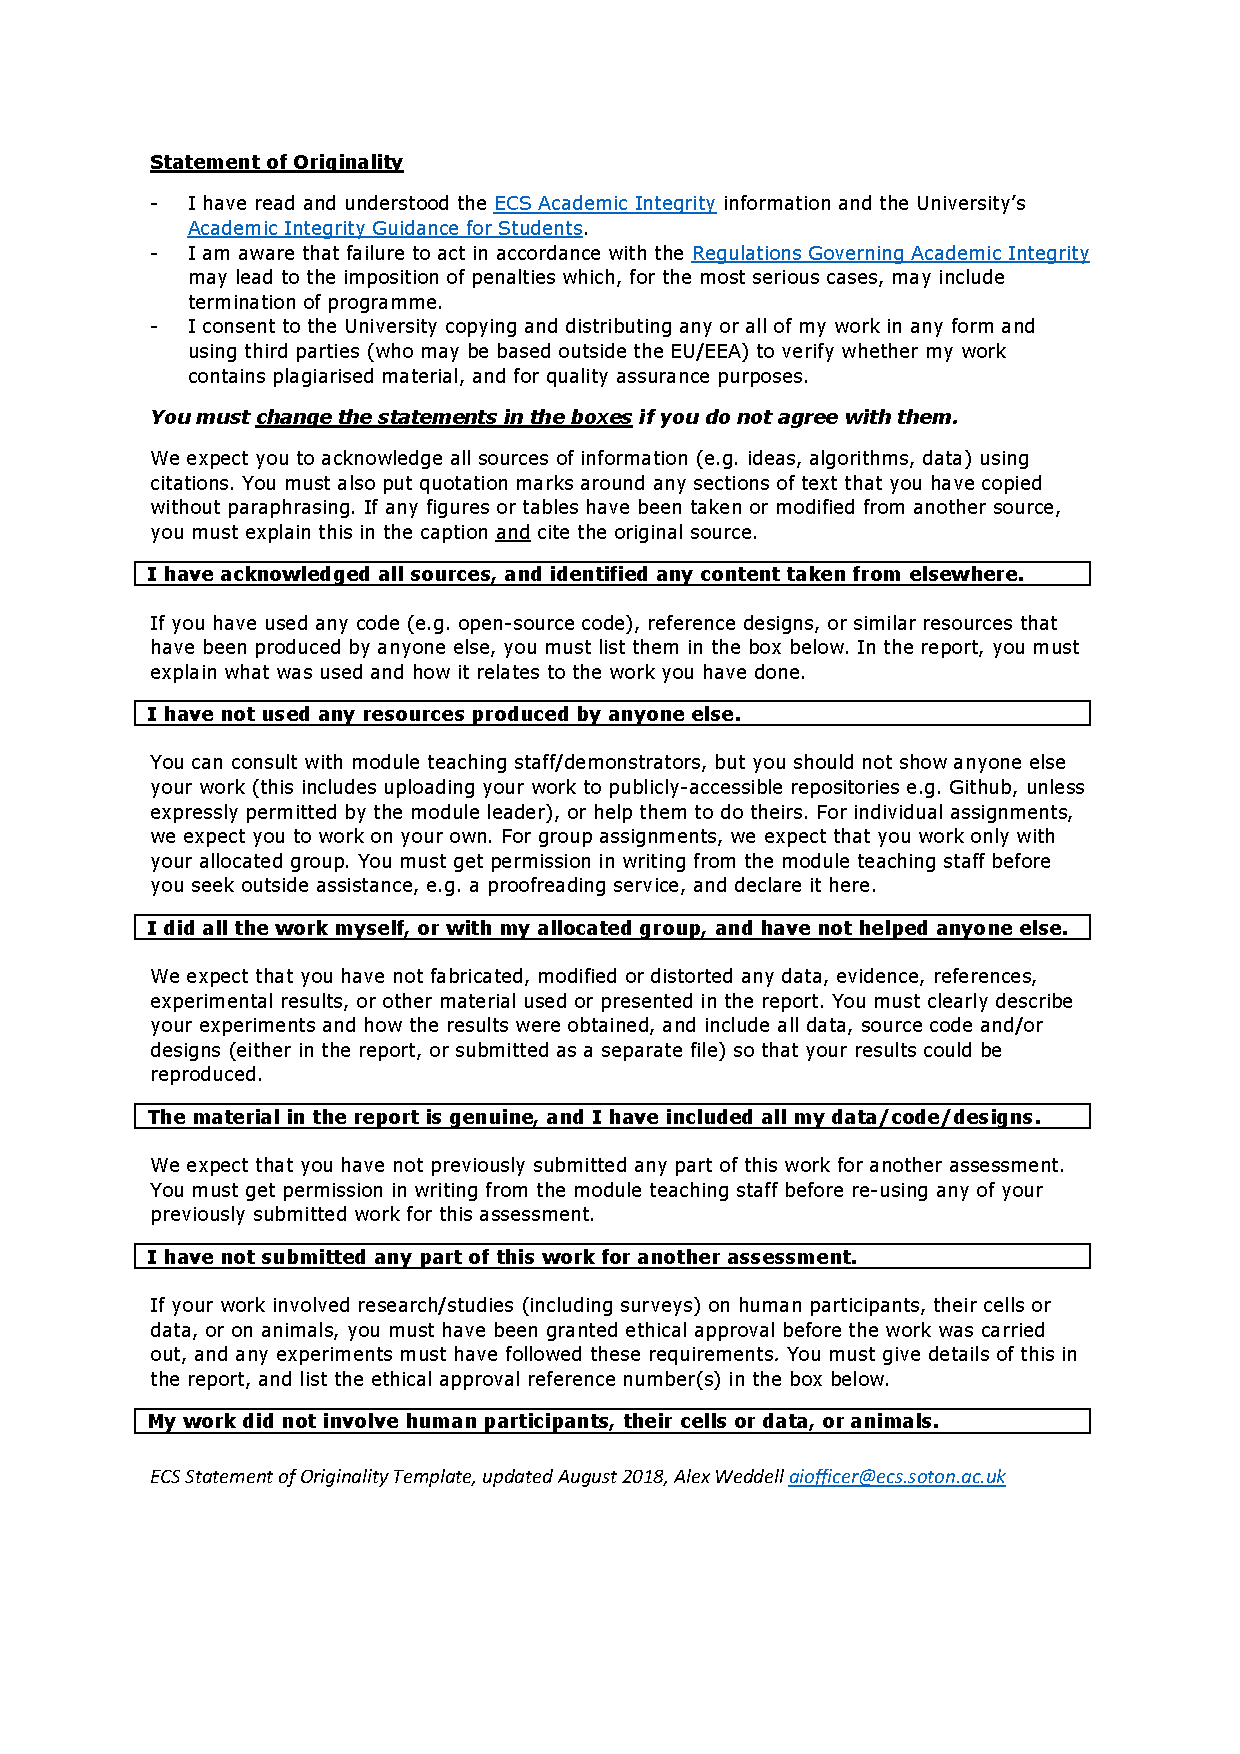
\includepdf[offset=25mm -30mm]{soo.pdf}
\tableofcontents
\listoffigures
\listoftables
% \lstlistoflistings
% \listofsymbols{ll}{$w$ & The weight vector}

\mainmatter
%% ----------------------------------------------------------------
%% ----------------------------------------------------------------
%% Introduction.tex
%% ---------------------------------------------------------------- 




\chapter{Introduction} \label{Chapter:Introduction}
% 区块链技术自发明以来就饱受争议,主要的争议点在于实际应用少,同时虚拟货币需要消耗大量的电力来进行挖矿,而目前全球电力的主要供应来源依然是化石能源,在用有限的化石能源电力时会产生大量排放。各国近年不停的推出严厉的排放政策以期缓解全球变暖以及化石能源枯竭的趋势,在这种背景下,碳排放市场和清洁能源交易逐渐走进人们的眼中,本项目旨在利用区块链技术实现一个无需挖矿的清洁能源电力交易平台,使它具备清洁能源以及其清洁积分交易的功能,使得普通人可以认购清洁能源证书以获取清洁能源积分,并且最后可以将清洁能源积分售卖给需要清洁能源积分的工厂从而形成一个良性的循环,吸引更多普通人参与这种环保行动以达到减少排放且能获得一定的收益的目的。
Blockchain technology has been controversial since its invention, the main point of contention is that there are not many practical applications, while cryptocurrencies need to consume a lot of power for mining \cite{disadvantagecrypto}, and the main source of global power supply is still fossil energy, which generates a lot of emissions when using limited fossil energy power\cite{QI2020115049}. In recent years, countries have been launching severe emission policies to alleviate global warming and the trend of fossil energy depletion, in this context, carbon emission market and clean energy trading gradually come into the eyes of people.

This project aims to use blockchain technology to realize a clean energy power trading platform without mining, so that it has the function of clean power and its clean power points trading. In the system, ordinary people can subscribe to clean energy certificates to obtain clean power points, and finally sell clean power points to factories that need to get emission rights by clean power points. In this way, people contribute to energy saving and emission reduction through clean power trading, while gaining a little profit, forming a virtuous circle of environmental action and promoting the popularity of clean power.

\section{Climate Problem}
As climate and environmental problems are becoming more and more serious, in order to protect the home that human beings depend on, countries have proposed their own schedule of carbon neutrality and carbon peaking in their respective government work reports, and the Japanese government proposed to achieve carbon neutrality by 2050 in October 2020\cite{japanesereport}. The Chinese government has also set a specific time frame for carbon peaking and carbon neutrality in the government work report \cite{chinareport}. According to Zhang \cite{Zhang2020}, the measure of carbon emissions trading for manufacturing companies has been effective in reducing carbon emissions in China for many years, with car companies producing low-emission or no-emission products, such as Tesla and BYD, making huge profits from the sale of carbon emission targets, and car companies producing high-emission products, such as Volkswagen and Geely, actively developing low-emission products and promoting technological progress. Thus,a multi-win situation has been achieved by emission market, however, complete carbon neutrality is a universal goal that requires the participation of everyone, so it is necessary to consider how to allow ordinary citizens to participate in the carbon emissions trading system. The production of electricity accounts for a large proportion of greenhouse gas emissions \cite{Zhu2020}, and electricity is something that everyone touches every day, and as fossil energy sources shrink and become more expensive \cite{Li2021}, clean electricity is gaining attention and is gradually being grid-connected and used on a large scale \cite{Sifat2019}. Therefore, clean power trading is a field in which everyone can participate.

\section{Power Internet}
Based on the concept of Internet Plus \cite{internetplus2016}, China has developed a well-developed power trading system in recent years \cite{energyinternet2015}, which refers to the use of Internet thinking and technology to transform the traditional power industry in order to achieve the deep integration of the Internet with power production, transmission, storage, consumption and power markets \cite{defenergyinternet}, and to create an power ecosystem with equal participation, common construction and governance, and collaborative operation. Among the new generation of information and communication technologies, blockchain technology, as a new distributed infrastructure and bookkeeping technology, can provide a trust basis for multi-party collaboration in the power Internet with its clever technical design and data governance \cite{Bao2020}.

\section{Blockchain Application}
The technical characteristics of blockchain have some similarity with the concept of power Internet, and both embody the ideas of decentralization and autonomous synergy, with the trend of intelligence and contractualization, and both can promote the establishment of market-based platforms \cite{Nofer2017}. Therefore, in recent years, there have been more and more theoretical and practical studies focusing on the application of blockchain technology in the power Internet. The literature \cite{summaryblockchian2019} summarized the typical application scenarios of blockchain in the fields of power supply, transmission, distribution, consumption and trading, and pointed out that blockchain would be the first to be applied in the field of power trading. The literature \cite{blockchainapplication2021} summarized the applications of blockchain technology in the fields of distributed power trading, data management and information security, carbon emission rights certification and green certificate trading, and concluded that scenarios such as distributed power trading are the most priority application areas for development and promotion. The literature \cite{Thu2020} introduced the current engineering status of blockchain+power applications at home and abroad, and pointed out that blockchain has unique advantages when used to solve the problems of renewable power consumption, distributed power trading, and lack of trust among multi-interest entities.



% You probably found all the files from \cite{Gunn:2001:pdflatex}.
% \tref{Table:tabex} illustrates the results of my work.
% \begin{table}[!htb]
%   \centering
%   \begin{tabular}{cc}
%   \toprule
%   \textbf{Training Error} & \textbf{Testing Error}\\
%   \midrule
%   0 & $\infty$\\
%   \bottomrule
%   \end{tabular}
%   \caption{The Results}
%   \label{Table:tabex}
% \end{table}

% \fref{Figure:figex} shows why this is the case.
% \begin{figure}[!htb]
%   \centering
%   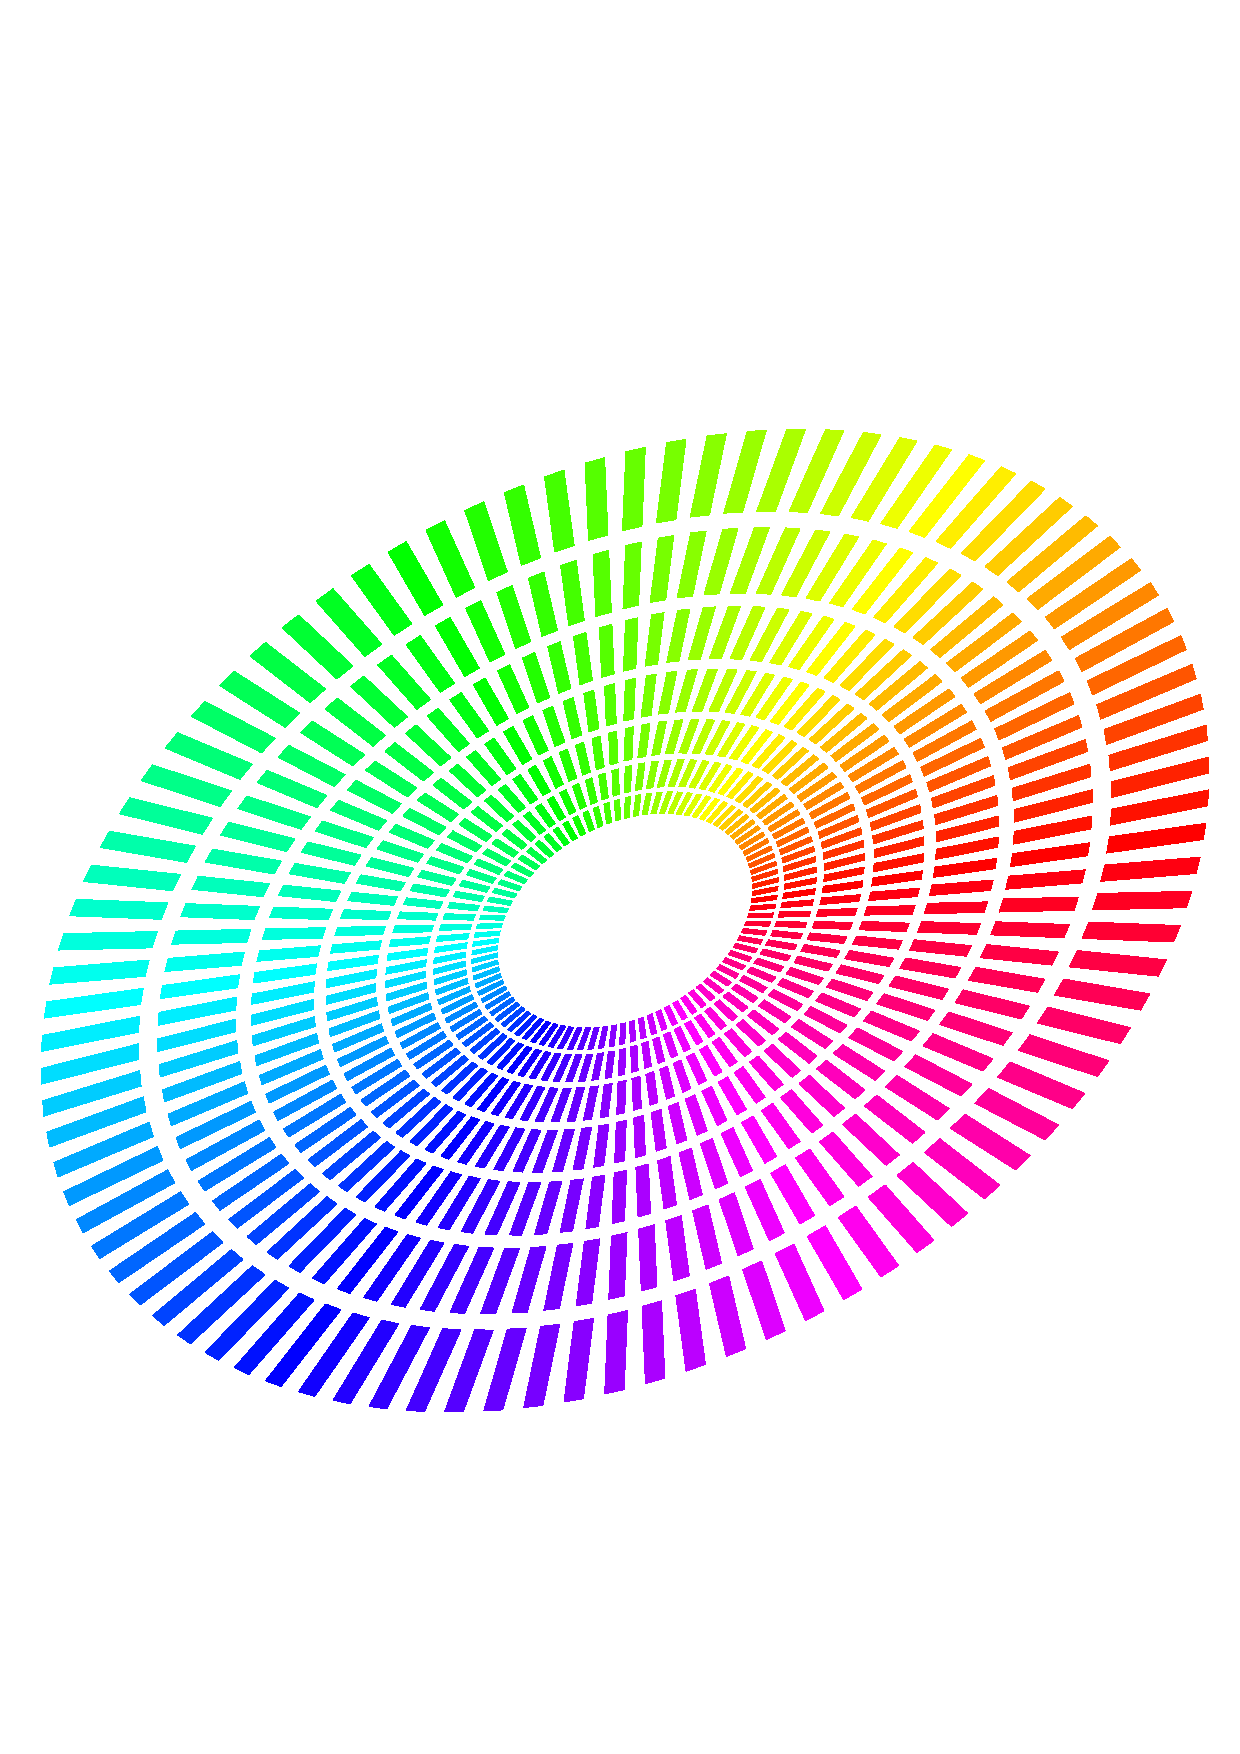
\includegraphics[width=8cm]{figure}
%   \caption{A colourful picture.}
%   \label{Figure:figex}
% \end{figure}

% This page shows you a subfigure example in \fref{Figure:figsubex}.
% \begin{figure}[!htb]
%   \centering
%   \subfigure[The left caption]{
%     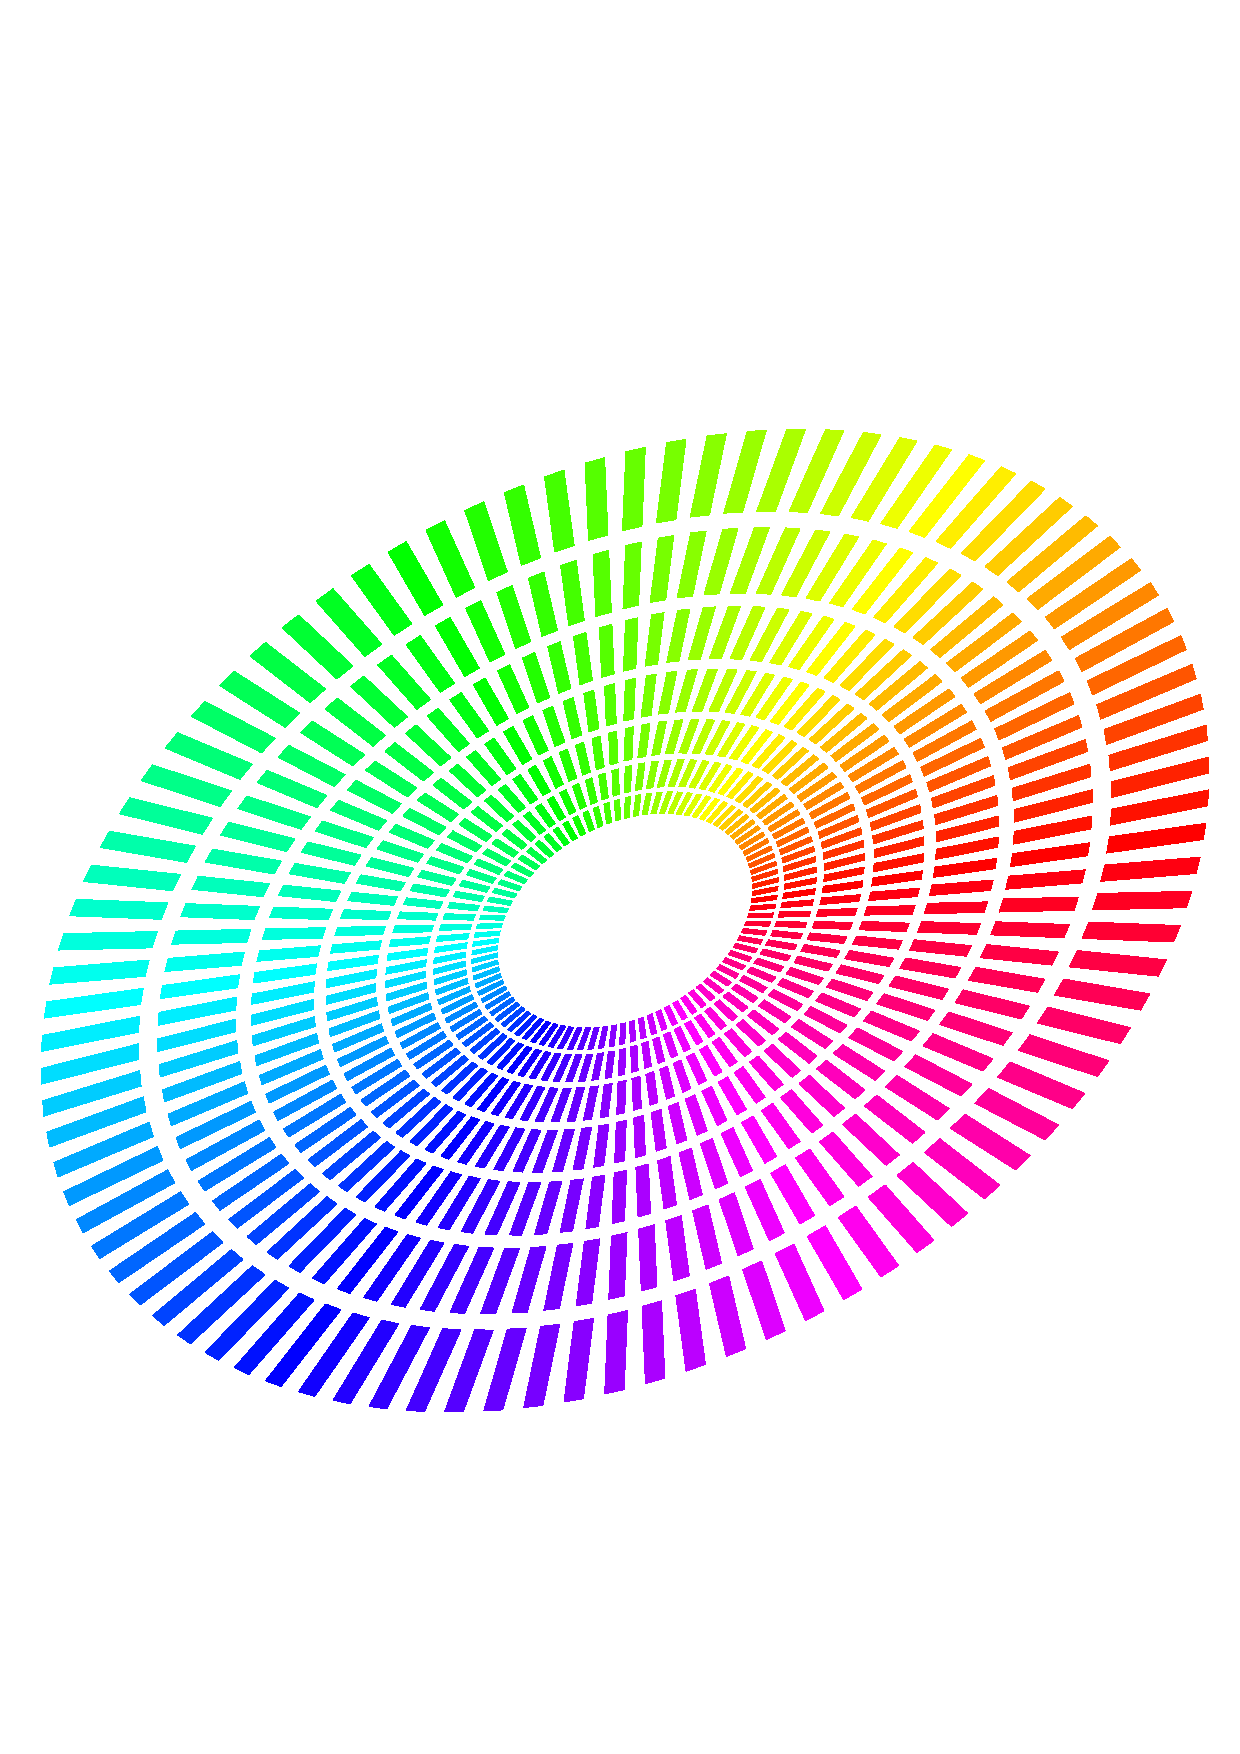
\includegraphics[width=4.2cm]{figure}
%     \label{Figure:figsubex:left}
%   }
%   \subfigure[The right caption]{
%     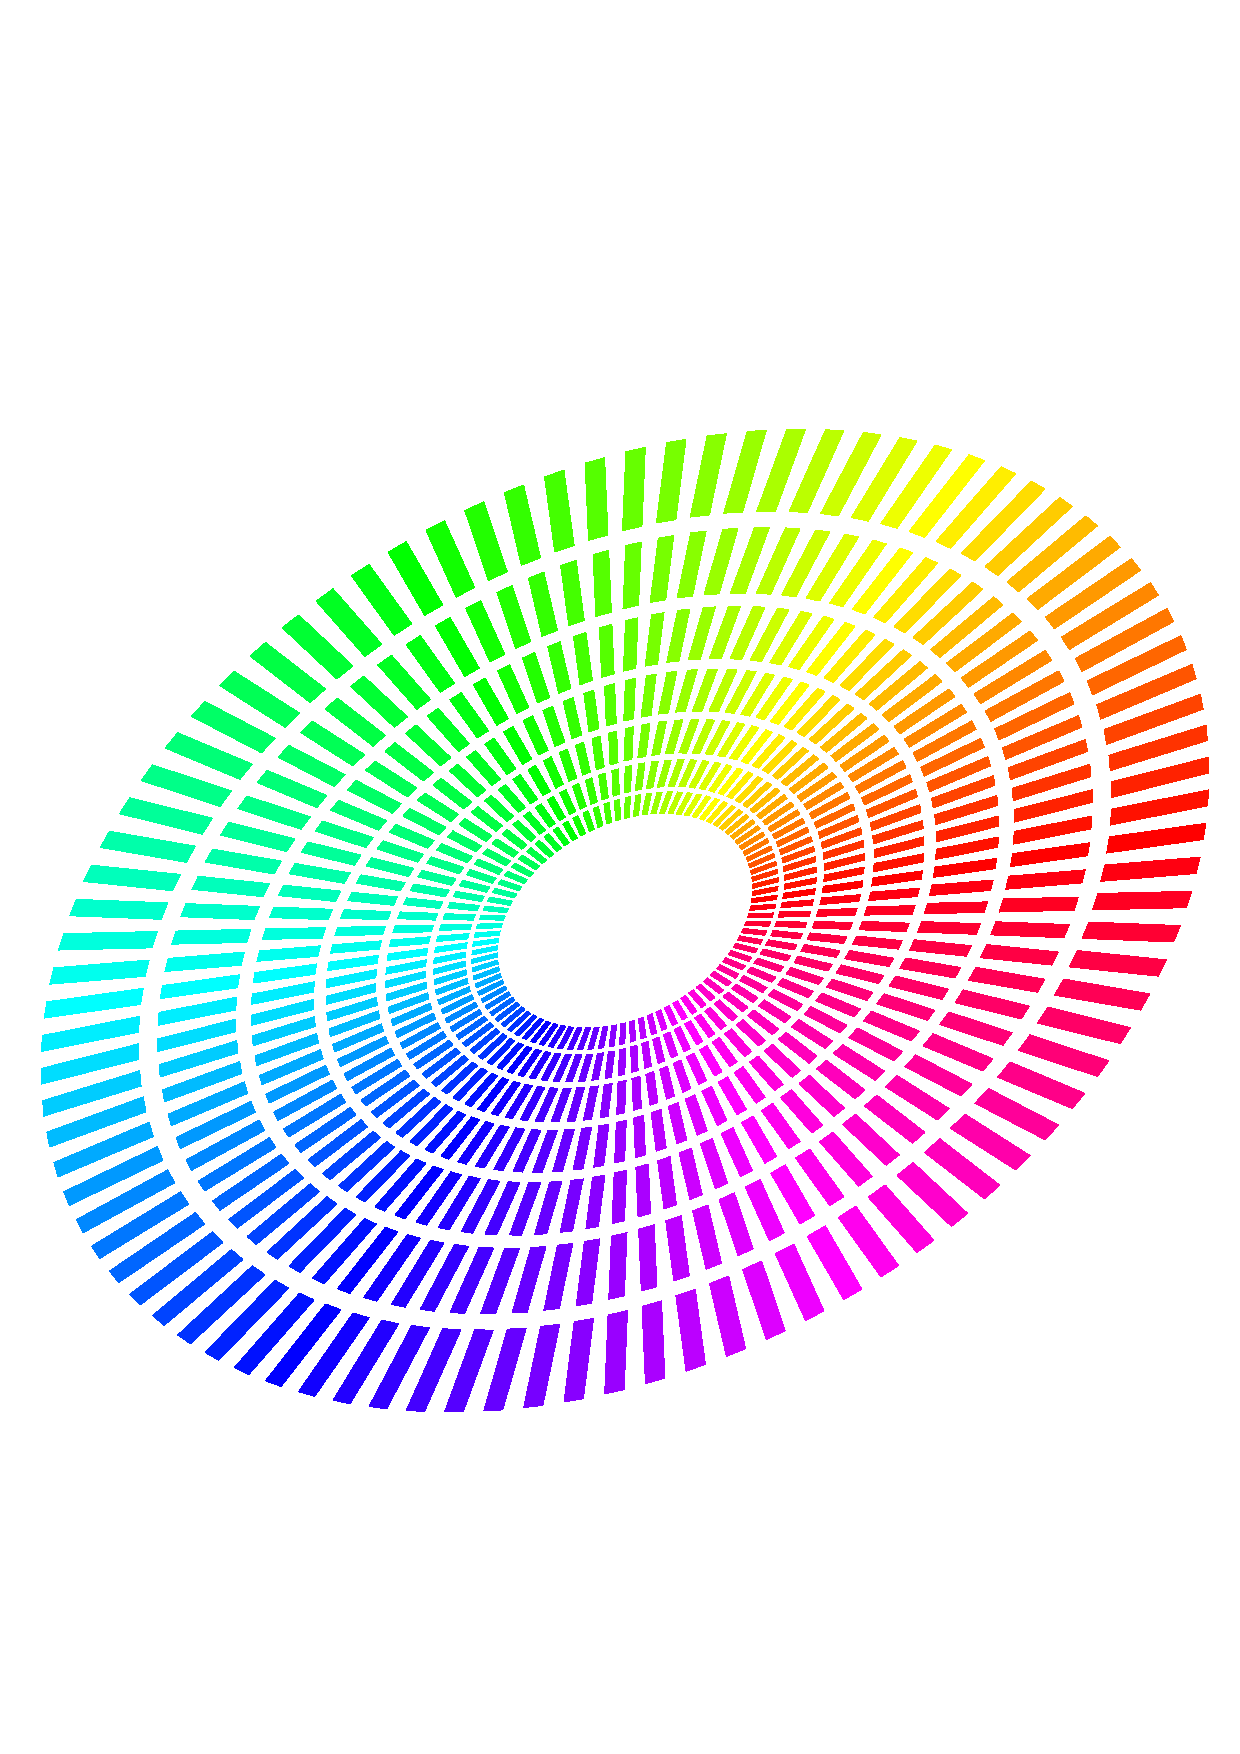
\includegraphics[width=4.2cm]{figure}
%     \label{Figure:figsubex:right}
%   }
%   \caption{A doubly colourful picture.}
%   \label{Figure:figsubex}
% \end{figure}

\chapter{Literature Review} \label{chapter:literature}
% 本项目想要实现的系统涉及碳排放市场,电力交易以及区块链技术,需要阅读大量相关文献,本章节会对涉及到的文献进行总结并对项目的可行性进行讨论。
The system that this project aims to implement involves carbon emission market, electricity trading and blockchain technology, which requires a lot of reading of related literature. This chapter will summarize the literature involved and discuss the feasibility of the project.
\section{Carbon Emissions Trading}
The Emissions Trading System (ETS) is a market-oriented tool launched by governments to reduce greenhouse gas emissions\cite{Han580003}. For every ton of greenhouse gas (usually carbon dioxide) emitted by a company in the carbon trading system emissions (usually carbon dioxide), a unit of carbon allowances is required. Companies can acquire or buy these emissions allowances, and they can also trade them with other companies. Currently, there are 17 carbon trading systems operating on four continents. The total cumulative regional GDP covered by carbon trading systems now accounts for 40\% of global GDP \cite{ZHAO20161229}.
\subsection{Participants of Carbon Emission Trading}
% 根据角色不同,目前碳排放交易的参与者可以分为政府,控制排放的企业,减少排放的企业,他们的具体界定如下:
% 政府:是市场监管者,它通过立法的形式明确碳市场的基本运行规则,如总量配额分配方法等。
% 控排企业:行业内年度温室气体排放量达到 2.6 万吨二氧化碳当量(综合能源消费量约 1 万吨标准煤)及以上的企业或者其他经济组织。
% 减排企业:卖出多余配额或生产CER。光伏、风电、生物质能供热及发电等项目均可开发出CCER,不过2017年3月17日,国家发改委发布公告,宣布暂停有关CCER方法学、项目、减排量、审定与核证机构交易机构备案的申请,待《暂行办法》修订完成并发布后,再依据新办法受理。目前,CCER上述相关工作仍处于暂停状态。
%其中控制排放的企业包含发电,供热,商业航空,以及炼油厂、钢铁厂、及生产铁、铝、其他金属、水泥、石灰、玻璃、陶瓷、纸浆、纸张、纸板、酸液和大批量有机化学品能源密集型的工业等
According to the different roles, the current participants of carbon emissions trading can be divided into government, enterprises controlling emissions, and enterprises reducing emissions, and they are defined as \tref{Table:tabRoleAndRes} \cite{ZHAO20171}:
\begin{table}[!htb]
    \centering
    \resizebox{\textwidth}{!}{
        \begin{tabular}{m{7cm}m{7cm}}
    \toprule
        \textbf{Role} & \textbf{Responsibilities} \\ \midrule
        Government & It is the regulator of the market, which specifies the basic operating rules of the carbon market through legislation, such as the method of allocating total allowances. \\ \midrule
        Emission-controlling enterprises & Enterprises or other economic organizations in the industry with annual greenhouse gas emissions of 26,000 tons of carbon dioxide equivalent (integrated energy consumption of about 10,000 tons of standard coal) and above. \\ \midrule
        Emission reduction enterprises & Sell excess allowances or produce emission credits. Emission credits can be developed by photovoltaic, wind power, biomass heating and power generation projects. \\
    \bottomrule
    \end{tabular}
    }
    \caption{The role and responsibilities in emission market}
    \label{Table:tabRoleAndRes}
\end{table}


Among the companies that need to control emissions are power generation, heating, commercial aviation, and refineries, steel plants, and energy-intensive industries producing iron, aluminum, other metals, cement, lime, glass, ceramics, pulp, paper, cardboard, acids, and high-volume organic chemicals \cite{YUYIN2018675}.

\subsection{Benefits and Problems of Carbon Emission Trading}
% 碳排放交易的优点如下:
% 1.碳排放交易保证环境效益:通过设定绝对总量并控制实际排放量,可有效实现减排领域的环境目标。就此而言,碳交易体系提供了其他政策工具所不具备的优点。以碳税为例,监管机构可通过征税保持价格稳定,但无法保证体系内的总排放量水平。补贴、标准以及监管法规等工具主要针对排放强度,效果存在不确定因素。相比之下,碳排放交易体系则控制总排放量,可保证实现减排目标。
% 2.碳排放交易保证成本效益:碳交易体系可以最低的经济成本实现既定减排目标。该体系主要通过对企业提供灵活性安排其减排时间和地点,来实现成本效益。各实体可选择经济效益最高的减排措施。在低成本减排方案不足的情况下,亦可选择在市场上购买配额。购买配额意味着一家企业正在资助另一家减排成本更低的企业实施减排。
% 3.碳排放交易提供经济灵活性:碳交易体系内根据当前经济状况调整碳价。若经济增长、排放量上升,配额价格将走高。经济增速放缓期间,价格则随产量和消费量减少而下降。可将碳排放交易体系视为经济风向标:经济强劲发展且能够投资低碳减排领域的时期,该体系可为开展减排工作提供更多激励。经济增速放缓时期,该体系设定的排放价格则相应下降。
% 4.实行碳排放交易体系可进一步加快开发、普及和应用低碳技术:通过设定长期总量,碳排放交易提供了长期价格信号,同时为私人投资开发和应用低排放/零排放技术提供了重要激励,从而降低了未来减排领域的宏观经济成本。此外,强劲的价格信号也有助于在市场参与者中间普及低排放/零排放技术。
% 5.碳交易制度为不同地区减排体系链接和减排合作提供可能性:通过碳交易体系的链接从而形成更广大的市场,有助于增加符合成本效益的减排选择,提高市场流动性。

\tref{Table:advofcarbonemision} shows the advantages of carbon emissions trading market\cite{JIA2020120187}.
\begin{table}[!htb]
    \centering
    \resizebox{\textwidth}{!}{
    \begin{tabular}{m{4cm}m{10cm}}
    \toprule
        \textbf{Advantages} & \textbf{Disadvantages} \\ \midrule
        High environmental benefits & High access threshold\\ \midrule
        High Cost-effectiveness &  Low marketability \\ \midrule
        High economic flexibility & Poor traceability\\ \midrule
        Accelerated low-carbon technologies & Carbon emission management for production materials (e.g. electricity) is not systematic \\ \midrule
        Compatibility to other fields and regions & \\ 
        \bottomrule
    \end{tabular}
    }
    \caption{Advantages and disadvantages of carbon emission market}
    \label{Table:advofcarbonemision}
\end{table}

\section{Blockchain}
% 区块链可以被看作是一个公共账本,其中所有承诺的交易都被储存起来,并在所有参与的可信方之间共享。它使数据或价值项目在两方之间转移,同时消除了对第三方促进转移的需要。
% 区块链的第一个公共使用案例是比特币。比特币是一种点对点的加密货币,它使用一个公共账本来记录所有的交易。第一笔比特币交易发生在2009年1月12日,中本聪和哈尔-芬尼之间。这笔第一笔交易来自中本聪的比特币地址1A1zP1eP5QGefi2DMPTfTL5SLmv7DivfNa,在创世区块(区块链网络的第一个区块)中发现。 \`footnote{\url{ https://news.bitcoin.com/eight-historic-bitcoin-transactions/}}。
% 众所周知,比特币是由中本聪开发的,详见他在2008年撰写的一篇名为《比特币:一个点对点的电子现金系统》的论文~\cite{nakamoto2019bitcoin}。
% 比特币因 "丝绸之路 "而流行,这是一个以销售非法毒品而闻名的在线黑市,使用加密货币进行匿名支付~cite{fleder2015bitcoin}。记录在区块链公共账本中的交易是永久性和不可改变的,发送方和接收方只能通过加密密钥来识别。
% 不变性是区块链的关键基石之一,它保证了存储在分布式账本中的数据的不可抵赖性和完整性。假设今天你从任何公开的比特币交易网站,如BitRef.com、Bit.com或Blockchain.com,查询中本聪的比特币地址,1A1zP1eP5QGefi2DMPTfTL5SLmv7DivfNa,你会得到从2009年第一笔交易到现在通过该比特币地址进行的所有交易。在撰写这篇论文时(2020年8月22日),这个比特币地址共有488笔交易,图2.1描述的是第一笔交易
%  此外,执法机构一直在依靠区块链记录的不变性,对通过互联网进行的非法支付交易进行调查。一个例子是丝绸之路的主谋Russ Ulbricht的案件,联邦陪审团以贩毒和洗钱的罪名判处他终身监禁,因为他的比特币地址是非法丝绸之路在线交易的主要受益人。
% 值得注意的是,即使在2013年丝绸之路被关闭后,丝绸之路毒品交易的所有比特币加密货币交易仍可在区块链上找到。这进一步证明,交易一旦记录在区块链账本上,就是永久的、不可更改的。在本文的设计和实施部分,我们将研究区块链的这种不可变性特征在我们的原型物联网安全和节能系统中为Gated社区提供的好处。
% 区块链技术最近已经从众所周知的加密货币支付平台发展成为一种可以可靠地用于政府、金融机构和企业实现去中心化应用的技术。


% \par区块链,可能是当下最有前景又充满分歧的技术与经济趋势。它给数字世界带来了“价值表示”和“价值转移”两项全新的基础功能。其潜力正在显现出来,但当下它又处于朦胧与野蛮生长的阶段。对比互联网的发展史,现在的区块链可能相当于1994年的互联网,即互联网刚刚进入大众视野的时期,那也是第一波互联网革命萌芽的时期。谷歌、亚马逊、Facebook、腾讯、阿里巴巴、优步、滴滴,甚至现在市值超万亿的苹果都得益于那一时刻。现在区块链技术可能带来互联网的二次革命,把互联网从“信息互联网”带向“价值互联网”。在区块链的对照之下,人们发现,最初被形象地称为“信息高速公路”的互联网处理的是“信息”,而区块链能处理的是“价值”。
% 众所周知,区块链的第一个应用案例是中本聪所开发的比特币,具体技术细节详见他的比特币白皮书[1],2009年1月3日,在位于芬兰赫尔辛基的服务器上,至今匿名的神秘技术极客中本聪生成了第一个比特币区块,即所谓的比特币创世区块(genesis block)。在创世区块的备注中,中本聪写入了当天英国《泰晤士报》的头版头条标题:“The Times 03/Jan/2009 Chancellor on brink of second bailout for banks”。在生成创世区块时,按他自己设定的规则,中本聪获得了 50 个比特币奖励,这是最早的 50个比特币。从创始区块开始,在比特币的账本上每10分钟就有新的数据区块被增加上去,新的比特币被凭空发行出来。比特币的去中心网络开始运转,扩展到现在的由数万个节点组成的全球网络。在比特币的创世时刻,它的三个组成部分都出现了,即加密数字货币、分布式账本、去中心网络。随着比特币的流行,它的分布式账本和去中心网络被人们提取出来,组成了区块链技术,所以,一种安全共享的去中心化的数据账本这一说法成为了目前公认的区块链定义[2]。区块链技术最近已经从众所周知的加密货币支付平台发展成为一种可以可靠地用于政府、金融机构和企业实现去中心化应用的技术[3]。

Blockchain is the most controversial but also the most rapidly developing technology today\cite{Blockchaintechnologyprinciplesandapplications}. For the digital world, what it does is create two new functions: "value representation" and "value transfer". The real role of blockchain has been discovered and practically applied.\cite{Andolfatto2018}. As the report said\cite{FRIZZOBARKER2020102029}, blockchain will transfer Internet from information world to value world.

The first known use case for blockchain was Bitcoin, developed by Satoshi Nakamoto, as detailed in his Bitcoin white paper \cite{nakamoto2019bitcoin}. At the moment of Bitcoin's creation, all three of its components emerged: the cryptographic digital currency, the distributed ledger, and the decentralized network. With the popularity of Bitcoin, its distributed ledger and decentralized network were extracted to form the blockchain technology, so the phrase a secure shared decentralized data ledger became the currently accepted definition of blockchain \cite{Ammous2016}. In recent years, blockchain technology has evolved through continuous development from a controversial technology closely tied to the term cryptocurrency to a new tool to help governments and enterprises achieve tighter and more efficient supply chains and information management\cite{8343163}.

\subsection{The underlying technology of blockchain}
% 去中心化信任:很多企业之所以采用区块链技术而不是其他数据存储技术,主要原因就是区块链不依赖中央权威就能保证数据完整性,即基于可靠数据实现去中心化信任。
% 区块:区块链顾名思义就是将数据存储在区块中,然后每一个区块都与前一个区块连接,组成链状结构。它仅支持添加(附加)新的区块,一旦添加,就无法修改或删除。
% 共识算法:共识算法负责区块链系统内的规则执行。当各参与方为区块链设置规则后,共识算法将确保各方遵守这些规则。
% 区块链节点:区块链节点负责存储数据区块,是区块链中的存储单元,可保持数据同步和始终处于最新状态。任意节点都可以快速确定是否有区块发生了变更。当一个新的全节点加入区块链网络时,它会下载当前链上所有区块的副本。而当新节点与其他节点同步并更新至最新的区块链版本后,它可以像其他节点一样接收任意的新区块。
% 区块链节点可分为两大类:

% 全节点:存储区块链的完整副本。
% 轻节点:仅存储最新区块且可在用户需要时请求较旧的区块。
% 区块链的分类
% 公共区块链:任何人都可以不受限制地加入公共或无许可区块链网络。在现实中,绝大多数类型的加密货币都在由规则或共识算法控制的公共区块链上运行。
% 许可区块链:专有或许可区块链允许企业控制哪些人可以访问区块链数据,即只有获得授权的用户才能访问特定数据集。Oracle 区块链平台就属于许可区块链。
% 区块链系统的基础技术构成为去中心化信任,区块,共识机制,节点,他们的具体作用如\tref{Table:partsofblocks}所示,其中,节点又可以分为全节点和轻节点,全节点承担保存整个区块链完整数据的任务,轻节点只负责存储近期的数据。区块链也可以分为公链和许可链,公链人人可以参与,而许可链仅允许受到特定许可的人或者机构参与。
The basic technical components of the blockchain system are decentralized trust, blocks, consensus mechanisms, and nodes\cite{LIM2021107133}, whose specific roles are shown in \tref{Table:partsofblocks}, where nodes can be divided into full nodes and light nodes, with full nodes undertaking the task of storing the complete data of the entire blockchain and light nodes only storing recent data. Blockchains can also be divided into public chains and permission chains\cite{permissionedandpublicblockchain}, where public chains are available to everyone, while permission chains only allow participation by people or institutions with specific permission.
\begin{table}[H]
    \centering
    \resizebox{\textwidth}{!}{
    \begin{tabular}{m{3cm}m{11cm}}
    \toprule
        \textbf{Technology} & \textbf{Description} \\ \midrule
        Decentralized trust & Guarantee data integrity without relying on central authority \\ \midrule
        Block & Stores data, once stored, can not be changed \\ \midrule
        Consensus mechanism & Ensure that all nodes follow the same rules to save the same data \\ \midrule
        Node & Stores blocks of data and it is the storage unit in the blockchain that keep data synchronized and always up-to-date \\
    \bottomrule
    \end{tabular}
    }

    \caption{Parts of a blockchain system}
    \label{Table:partsofblocks}
\end{table}

\subsection{Features comparison between blockchain technologies}
% 随着区块链从业人员以及参与企业的日渐增多,许多区块链的基础工具出现了,比较有代表性的两个是Hyper Ledger和以太坊,他们的区别列在了表1中。经过对比,本项目选择Hyper Ledger Fabric作为区块链工具,原因是本项目的性质是私链,对于私链而言,Hyper Ledger Fabric无疑是更多企业在进行私链开发时的选择,且无需挖矿。
With the increasing number of blockchain practitioners as well as participating companies, many blockchain-based tools have emerged. Two of the more representative ones are Hyper Ledger Fabric and Ether\cite{comparisionethhyper}, and their differences are listed in \tref{Table:comparisionblockchain}. Through comparison, Hyper Ledger Fabric is chosen as the blockchain tool for this project because the character of this project is private chain, and for private chain, Hyper Ledger Fabric is undoubtedly the choice for more enterprises when they do private chain development and no mining is required.

\begin{table}[H]
\centering
\resizebox{\textwidth}{!}{
\begin{tabular}{lm{5cm}m{5cm}}
\toprule
\textbf{Features} & \textbf{Hyperledger} & \textbf{Ethereum}                                                            \\ \midrule
                           & Preferred platform for B2B businesses             & Platform for B2C bussinesses and generalized applicaitons           \\ \midrule
Confidential               & Confidential transactions                         & Transparent                                                         \\ \midrule
Mode of Peer Participation & Private and Permissioned Netword                  & Public/Private and permissionless netword                           \\ \midrule
Consensus Mechanism        & Pluggable Consensus Algorithm: No mining required & PoW Algorithm: Consensus is reached by mining                       \\ \midrule
Programming Language       & Chaincode written in Golang                       & Smart Contracts written in solidity(Implements by golang in ETH2.0) \\ \midrule
Crypto currency             & No built-in crypto currency                        & Built-in crypto currency called Ether\\    
\bottomrule
\end{tabular}
}

\caption{Comparision between blockchain technologies}
\label{Table:comparisionblockchain}
\end{table}


\subsection{Consensus Mechanisms}
% 如上一部分所述,区块链系统成立的基础其实是共识机制,共识机制分为两大类,拜占庭容错和非拜占庭容错,最常用到的是PoW,PoS,PoA,DPoS,PBFT,Raft,他们具体的概述被列在了\tref{Table:consensus}中。在选择共识机制时,首先排除PoW,PoS以及DPoS,因为他们都需要挖矿,与项目初衷不符,接着排除Paxos,因为它几乎没有软件实现,PoA也因为不符合项目要求而排除,最后在Kafka和Raft中选择了Raft是因为Kafka配置繁琐,稳定性低。
According to the description of blockchain before, the basis for the successful establishment and stable performance of blockchain systems is actually the consensus mechanism, which is divided into two main categories, Byzantine fault tolerance and non-Byzantine fault tolerance, the most commonly used ones are PoW, PoS, PoA, DPoS, PBFT, Raft \cite{Mingxiao2017}, and their specific overviews are listed in \tref{Table:consensus}. When choosing the consensus mechanism, PoW, PoS and DPoS were excluded first because they all required mining, which was not in line with the original intention of the project, then Paxos was excluded because it had almost no software implementation, PoA was also excluded because it did not meet the requirements of the project, and finally Raft was chosen among Kafka and Raft because of the cumbersome configuration and low stability of Kafka.

\begin{table}[H]
\centering
\resizebox{\textwidth}{!}{
\begin{tabular}{cm{2cm}m{3cm}m{3cm}m{2cm}m{2cm}}
\toprule
\textbf{Category}& \textbf{Name} & \textbf{Advantage} & \textbf{Disadvantage} & \textbf{Mining} & \textbf{Example}                               \\ 
\midrule
\multirow{5}{*}{Byzantine fault tolerance}     & PoW   & Simple and easy to implement, high security                                                  & Environmentally unfriendly and heavily dependent on miners                     & Yes    & Bitcoin, Ethereum, Litecoin, Dogecoin \\ \cline{2-6} 
                                               & PoS   & Consensus reaching time and energy consumption less than PoW                                 & Easy to form monopolies and easily bifurcated                                  & Yes    & Ethereum, Peercoin, Nxt               \\ \cline{2-6} 
                                               & DPoS  & Fast to confirm transactions and low energy cost                                             & Have centralization and security risks                                         & Yes    & Steemit, EOS, Lisk, Ark               \\ \cline{2-6} 
                                               & PoA   & Perfect for private chains, fast to confirm transactions                                     & Sacrificing trustworthiness                                                    & No     & Ethereum, Kovan, testnet, VeChain     \\ \cline{2-6} 
                                               & PBFT  & Communication complexity O($n^{2}$), and effective                                           & Only applicable to permissionsed systems                                       & No     & Hyper Ledger Fabric                   \\ \midrule
\multirow{3}{*}{Non-Byzantine fault tolerance} & Paxos & Efficient, with rigorous mathematical proofs, well-designed systems and high fault tolerance & Engineering practice is difficult and only applicable to permissionsed systems & No     & -                                     \\ \cline{2-6} 
                                               & Kafka & Easy to realize and maintain                                                                 & Low security                                                                   & No     & Hyper Ledger Fabric                   \\ \cline{2-6} 
                                               & Raft  & Effective and easy to implement                                                              & Only applicable to permissioned systems                                        & No     & Hyper Ledger Fabric                   \\ 
\bottomrule
\end{tabular}
}
    \caption{Details of consensus mechanisms}
    \label{Table:consensus}
\end{table}

\section{Blockchain-based Power Trading Market}
% 现代社会正常运转无法离开电力,煤炭,石油,天然气都可以产生电力,但是电力进入电力市场需要有可以被人们接受的价格,否则便会无人问津,当前化石能源生产的电力成本随着各国对各行业的碳排放限制逐步增加,而清洁能源电力反而随着技术的更新迭代不断地降低了成本,但是清洁能源电力占据市场份额的步伐却没有预想中迅速,与其市场化程度低是有一定关系的\cite{renewableenergy}。
Modern society cannot function without power, coal, oil, natural gas can produce power, but power in the power market needs to have a price that people can accept, otherwise no one will ask for it. The current cost of power produced by fossil energy is gradually increasing with the tightening of carbon emission policies in various countries, while clean energy power with the iteration of technology continues to reduce the cost, but the pace of clean energy power to occupy the market share is not as fast as expected, and its low degree of marketization is somewhat related to \cite{renewableenergy}

% 区块链是电力行业市场化的一个理想工具,目前已经有许多的基于区块链的电力项目落地,并且运行良好,他们有不同的特性,具体的对比列在了\tref{Table:ComparePowerMarket}
Blockchain is an ideal tool for marketization in the power industry, and there are already many blockchain-based power projects on the ground and working well \cite{Jamil2021}, they have different characteristics, the specific comparison is listed in \tref{Table:ComparePowerMarket}.
\begin{table}[!htp]
\resizebox{\textwidth}{!}{
\begin{tabular}{lm{2cm}m{2cm}m{2cm}m{2cm}}
\toprule
\textbf{Platform} & \textbf{Pricing Mechanism} & \textbf{Consensus} & \textbf{Crypto Currency} & \textbf{Mining} \\ \midrule
NRG coin        & Yes               & PoW/PoS              & Yes             & Yes             \\ \midrule
Sunchain        & No                & PoW                  & No              & No              \\ \midrule
GridSingularity & No                & PoA                  & Yes             & Yes             \\ \midrule
Excrgy          & Yes               & PoS                  & Yes             & Yes             \\ \midrule
SolarCoin       & Yes               & PoS                  & Yes             & Yes             \\ \midrule
Pylon network   & Yes               & PoW                  & Yes             & Yes             \\ \midrule
Power Ledger    & Yes               & PoW/PoS              & Yes             & Yes             \\ \midrule
Proposed System & No                & PBFT                 & No              & No             \\
\bottomrule
\end{tabular}
}


\caption{Comparision between power blockchain project}
\label{Table:ComparePowerMarket}
\end{table}

\section{Disscussion}
% 从之前的文献可以知道,电力交易衍生品目前主要包括绿色电力证书和可再生能源过度消费证书。电力衍生品本身只具有金融属性,通常独立于现有电力市场进行交易。开发基于区块链技术的衍生品交易平台可以减少与现有系统数据库的交互,降低开发难度和开发成本,同时发挥技术的信任保障优势。例如,通过基于区块链的绿色电力证书和全民碳排放权交易系统,可以提高个人减排的积极性,为全球环境做出巨大贡献。目前还没有适合个人直接参与的区块链清洁能源电力认购项目,也没有个人可以参与的区块链碳交易项目,而随着人们环保意识的增强,全球气候有更加严峻的趋势。碳排放将成为一个重要的经济项目,甚至是一个金融项目,而企业碳排放交易已经实施了多年,效果很好,现在是时候借助区块链技术向个人开放碳交易市场,让更多人参与其中。综上所述,目前市场在个人清洁电力和碳排放交易领域是存在空白的,可以由此开发一个基于区块链的电力交易系统,填补这个空白。
From the previous literature, it is known that power trading derivatives currently include mainly green power certificates and renewable energy overconsumption certificates. Power derivatives themselves have only financial attributes and are usually traded independently of the existing power market. Developing a derivatives trading platform based on blockchain technology can reduce the interaction with the existing system database, reduce the development difficulty and development cost, and at the same time take advantage of the trust guarantee of the technology. For example, through blockchain-based green power certificates and a universal carbon trading system, individuals can be more motivated to reduce emissions and make great contributions to the global environment. At present, there is no blockchain clean energy power subscription project suitable for direct personal participation, nor is there a blockchain carbon trading project that individuals can participate in, but as the global climate has a more severe trend, people are increasingly aware of environmental protection. Carbon emission will become an important economic project, or even a financial project, while corporate carbon emission trading has been implemented for many years with good results, and now it is time to open the carbon trading market to individuals with the help of blockchain technology, so that more people can participate in it. To sum up, there is currently a gap in the market in the field of linking personal clean power and carbon emissions trading, and a blockchain-based power trading system can be developed as a result to fill this gap.


\chapter{Requirements Document} \label{chapter:requirement}
% 由于本项目偏向于实际开发,因此适用于软件工程通用流程,即需求分析,系统设计,详细设计,编码,测试,集成等流程,为了提高开发效率,还会引入敏捷开发的方法来进行需求的取舍,从而达到系统快速可用,快速迭代的目的。因此,本系统所有功能以及特性都基于本章的需求文档进行开发。
Since this project is oriented towards practical development, the common software engineering processes, i.e. requirements analysis, system design, detailed design, coding, testing, integration, will be applied. In order to improve development efficiency, agile development methods will be introduced to make requirements trade-offs so that the system will be available quickly and iterate quickly. Therefore, all functions and features of this system are developed based on the requirements document in this chapter.

\section{Persona Analysis}
% 在软件工程领域,为了编写高质量的需求文档,通常需要对系统的利益相关者进行采访,进而提取出用户故事,描述用户故事有许多方法,本文采用Persona方法进行表格陈列来叙述用户故事\cite{persona}。如\tref{Table:Persona}所见,本系统主要用户分为三类:普通用户,管理员,发电终端以及需要购买清洁能源积分的工厂老板。其中普通用户有着不同的身份背景,因此他们有不同的使用习惯以及不同的使用目标,例如将清洁能源积分视为投资标的;管理员的日常工作则是管理整个系统;工厂老板需要在这个系统中向用户以及发电终端购买清洁能源证书或者积分;最后,发电终端则需要在接收到订单的时候自动执行清洁能源证书发行
In the field of software engineering, in order to write high quality requirement documents, it is often necessary to interview the stakeholders of the system and then extract the user stories. There are many ways to describe the user stories, and in this paper, we use the Persona method for table display to narrate the user stories \cite{persona}. As seen in \tref{Table:Persona}, the main users of the system are divided into three categories: general users, administrators, power generation terminals, and factory owners who need to purchase clean power points. The common users have different backgrounds, so they have different habits and goals, for example, they may consider clean energy credits as an investment target; the administrator's daily work is to manage the system; the factory owners need to purchase clean energy certificates or credits from users and generation terminals in the system; and finally, the generation terminals need to automatically perform the task of issuing clean energy certificates when they receive orders. The plant owner needs to purchase clean power certificates or points from users and generation terminals.
\begin{table*}[!htb]
\centering
\resizebox{\textwidth}{!}{
\begin{tabular}{ccm{6cm}m{5cm}}
\toprule
\textbf{Persona} & \textbf{Avatar} & \textbf{User Info}& \textbf{User Scenarios}                                                                               \\ \midrule
Sam& 
\includegraphics[width=1cm]{img/user-avatar.png}
& Age:25-60 years old;Occupation:Any;Skills:Internet shopping,social networking;Characteristics:Concerned about new technology,care about environmental protection, have the desire to invest; Education level:High school or above.
& When topping up your metered account, you want to prioritize the purchase of clean power and earn clean power points when you use it.Want to be able to trade your Clean Power Points for useful items.You want your Clean Power Points to be appreciated and traded with others.\\ \midrule

Jone & 
\includegraphics[width=1cm]{img/boss.png}
	& Age:Any; Occupation:Factory manager;Skills:Internet shopping; Characteristics:Need carbon credits in exchange for production targets; Education:Any & When you top up your metered account, you can choose to purchase clean power first and earn clean power credits when you use clean power.You can use Clean Power Credits to exchange for carbon emission targets.You can use money to buy Clean Power Credits from regular electricity users in the market.You can sell your Clean Power Credits on the market.\\ \midrule
Shufu    & 
\includegraphics[width=1cm]{img/manager.png}
	& Occupation:System administrator; Skills:Basic computer professional skills; Characteristics:Rigorous, honest and serious;Education:Bachelor's degree or above in computer-related majors. & You can monitor the system operation information.You can make changes to the system operation configuration.It is possible to operate the orders of the system (shipping, cancellation)\\ \midrule
Generator&
\includegraphics[width=1cm]{img/generator.png}
	& Occupation: Power Generator& Clean power credits can be generated at the time of power generation. \\
	\bottomrule
\end{tabular}
}

\caption{Persona Table of the system}
\label{Table:Persona}
\end{table*}

\section{Function Requirements}
% 根据Persona所描述的用户故事,可以导出详细的需求列表,用户需求分为功能需求和非功能需求,功能需求表示系统或者系统中组件的行为和功能,可以表现为一组输入和输出,也可以表现为具体的事务处理流程,非功能需求是在功能需求的基础上对功能需求的具体实现提出的限制,包含安全需求,性能需求等,本节将详细描述系统的功能需求。
Based on the user story described by Persona, a detailed list of requirements can be derived. User requirements are divided into functional and non-functional requirements. Functional requirements represent the behavior and functions of the system or components in the system, which can be expressed as a set of inputs and outputs, or as a specific transaction processing flow, and non-functional requirements are the restrictions on the specific implementation of functional requirements based on the functional requirements. Contains security requirements, performance requirements and so on \cite{funcnonfuncreq}. This section will describe the functional requirements of the system in detail.
\subsection{Function Requirements of Users}
% 对于清洁电力用户而言,他们的功能要求应该包含登录,注册,购买清洁电力,用清洁电力积分购买系统内的礼物,出售或购买清洁电力,修改自己的个人信息,在购买清洁电力后,用户会获得清洁电力证书,证书可以被兑换成清洁电力积分,这一条是未列在需求表中的功能需求。具体的用户功能需求列在了\tref{Table:FRuser}
For Clean Power users, their functional requirements should include log in, register, buy Clean Power, use Clean Power Points to buy gifts in the system, sell or buy Clean Power Points, modify their personal information, and after buying Clean Power, the user will get a Clean Power certificate, which can be redeemed for Clean Power Points, which is a functional requirement not listed in the requirement table. The specific user functional requirements are listed in \tref{Table:FRuser}
\begin{table}[!htb]
\centering
\resizebox{\textwidth}{!}{
\begin{tabular}{cm{3cm}m{7cm}}
\toprule
\textbf{Function Requirement} & \textbf{Name} & \textbf{Description}                                                                                                                             \\ \midrule
FR-1                 & Login                            & User can login the system                                                                                                               \\ \midrule
FR-2                 & Register                         & User can register as a user                                                                                                             \\ \midrule
FR-3                 & Buy Clean Power and Clean Power Points   & User  can  buy  clean  power  and cleanpower points in market                                                                                   \\ \midrule
FR-4                 & Browse Market & Users can browse the Clean Power, Gifts, and Clean Power Points Marketplace where they can use Clean Power Points to purchase items and sell Clean Power Points \\ \midrule
FR-5                 & Buy Gifts by Clean Power Points  & Users can buy the items in clean power gifts market by Clean Power Points                                                                     \\ \midrule
FR-6                 & Sell Clean Power Points          & Users can sell Clean Power Points to factories or others                                                                                \\ \midrule
FR-7                 & Browse Personal Profile          & Users can see their personal information                                                                                                \\ \midrule
FR-8                 & Edit Personal Profile            & Users can edit their personal information \\
\bottomrule
\end{tabular}
}
\caption{Function requirements of users}
\label{Table:FRuser}
\end{table}

\subsection{Function Requirements of Power Generator}
% 对于发电终端而言,功能相对简单,只需要实现售出清洁电力,生成清洁电力证书,发送清洁电力积分的功能,具体功能需求列在了\tref{Table:frPower}
For the power generator terminal, the function is rather simple, it only needs to realize the function of selling clean power, generating clean power certificate and sending clean power points, the specific function requirements are listed in \tref{Table:frPower}
\begin{table}[H]
\centering
\resizebox{\textwidth}{!}{
\begin{tabular}{cm{3cm}m{7cm}}
\toprule
\textbf{Function Requirement} & \textbf{Name} & \textbf{Description}                                                                           \\ \midrule
FR-9                 & Generate Clean Power Certificate & A clean power generator can generate Clean Power Certificate when clean power is sold \\ \midrule
FR-10                & Sell the Clean Power        & A clean power generator can sell the clean power to consumer                          \\ \midrule
FR-11                & Send the Clean Power Points & When the clean power certificate is redeemed, the clean power point will be send     \\
\bottomrule
\end{tabular}
}
\caption{Function requirements of power generator}
\label{Table:frPower}
\end{table}

\subsection{Function Requirements of Factory}
% 对于工厂主而言,他们的核心需求与普通用户大致相同,具体需求列在了\tref{Table:frFact}
For factory owners, their core requirements are roughly the same as those of ordinary users, and the specific requirements are listed in the \tref{Table:frFact}
\begin{table}[!htb]
\resizebox{\textwidth}{!}{
\begin{tabular}{cm{3cm}m{7cm}}
\toprule
\textbf{Function Requirement} & \textbf{Name} & \textbf{Description}                                                                                                                            \\ \midrule
FR-12                 & Login                            & Factory can login the system                                                                                                               \\ \midrule
FR-13                 & Register                         & Factory can register as a factory                                                                                                             \\ \midrule
FR-14                 & Buy Clean Power Points                & Factories can buy clean power points                                                                                    \\ \midrule
FR-15                 & Transfer Clean Power Points to Emission Credits & Factories can transfer Clean Power Points to Emission Credits \\ \midrule
FR-16                 & Buy Goods by Clean Power Points  & Users can buy the items in clean power market by Clean Power Points                                                                     \\ 
\bottomrule      
\end{tabular}
}
\caption{Function requirements of factory}
\label{Table:frFact}
\end{table}

\section{Non-functional Requirements}
% 由于本系统中主要涉及电力交易以及积分交易活动,系统资产实质上是货币,所以对安全性和交易确认的快速性有一定的要求,因此,本节会详细地列出系统的安全需求和性能需求。
Since this system is mainly involved in power trading as well as point trading activities, and the system assets are basically currencies, there are certain requirements for security and fast transaction confirmation, so this section will list the security requirements and performance requirements of the system in detail.

\subsection{Security Requirements}
% 用户的安全需求需要基于安全的三要素:机密性,可用性,完整性(CIA)进行,因此为了维护CIA特性,需要满足诸如用户验证,访问控制,数据验证,强制登出,强制过期密码的功能,具体安全需求列在了\tref{Table:SecReq}
The security requirements of the system need to be based on the three elements of security: confidentiality, availability, and integrity (CIA)\cite{cia}. Therefore, in order to maintain the CIA features, functions such as user authentication, access control, data validation, mandatory logout, and mandatory password expiration need to be satisfied, and the specific security requirements are listed in \tref{Table:SecReq}.
\begin{table}[!htb]
\resizebox{\textwidth}{!}{
\begin{tabular}{cm{3cm}m{7cm}}
\toprule
\textbf{Security Requirement} & \textbf{Name} & \textbf{Description}   \\ \midrule                                        SR-1                 & Verify Identity of Users      & The system can identify the user(Visitor,Registered,Generator)                                                      \\ \midrule
SR-2                 & Verify Identity of Devices    & The system can identify the legal Devices(Power generation terminal, power interruption, malicious access terminal) \\ \midrule
SR-3                 & Verify Authorization of Users & The system can identify who can use the system                                                                      \\ \midrule
SR-4                 & Integrity of data             & Data in system should be encrypted and should not be modified or stolen by others                                   \\ \midrule
SR-5                 & Access control                & The system can identify the rights of different users to control the services and files they can access             \\ \midrule
SR-6                 & Input Validation              & All the Input in the system should be in the bound of the system and be valid.                                      \\ \midrule
SR-7                 & Monitor security reports      & All dangerous action in system should be monitored and reported                                                     \\ \midrule
SR-8                 & Enforce logout                & Login should be expired after a period                                                                              \\ \midrule
SR-9                 & Enforce changing password     & Password should be changed regularly                 \\ 
\bottomrule      
\end{tabular}
}
\caption{Security requirements of system}
\label{Table:SecReq}
\end{table}

\subsection{Performance Requirements}
% 由于系统涉及金钱交易,所以需要一定的时效性,因此对于系统加载速度,交易提交速度,交易被确认的速度有限制,具体描述列在了\tref{Table:PerfReq}
Since the system involves money transactions, it needs to be time-sensitive, so there are limits on how fast the system can load, how fast transactions can be submitted, and how fast transactions can be confirmed, as described in \tref{Table:PerfReq}
\begin{table}[H]
\resizebox{\textwidth}{!}{
\begin{tabular}{cm{3cm}m{7cm}}
\toprule
\textbf{Performance Requirement} & \textbf{Name} & \textbf{Description}   \\ \midrule                             PR-1                    & Loading speed     & Every page should be loaded in 5 seconds                                           \\ \midrule
PR-2                    & Trading speed     & Every transaction should be confirmed in 15 seconds                                \\ \midrule
PR-3                    & Concurrency Speed & The system should support more than a million people trading at the same time      \\ \midrule
PR-4                    & System Capacity   & The system should support over 100 billion transactions and over 100 million users \\ 
\bottomrule      
\end{tabular}
}
\caption{Performance requirements of system}
\label{Table:PerfReq}
\end{table}

\section{MoSCoW Analysis}
% 为了快速开发出系统,本项目选择敏捷开发方式。敏捷开发因为其快速成型,快速上线的特性,吸引着无开发者前赴后继地加入敏捷开发的大军,这种开发方法的最核心观念就是快速的开发原型,然后快速的进行迭代\cite{agile}。因此,下一步应该对需求进行分类,排序,从成本和时间等多维度及逆行考量进行优先级排序,优先开发必须有的功能,其次开发应该有的功能,以此类推,这就是MosCoW方法\cite{moscow}。在敏捷开发中,MoSCoW常常被用来对需求进行排序和筛选,本系统的需求排序和筛选结果列在了\tref{Table:moscow}
In order to develop the system quickly, this project chose the agile development approach. The core concept of this development method is to develop prototypes quickly and then iterate quickly\cite{agile}. Therefore, the next step should be to categorize and rank the requirements, prioritize them in terms of cost and time and other multi-dimensional and retrograde considerations, prioritize the features that must be developed, followed by the features that should be developed, and so on, which is the MosCoW approach \cite{moscow}. In agile development, MoSCoW is often used to sort and filter requirements, and the results of this system are listed in \tref{Table:Moscow}
The core concept of this development method is to develop prototypes quickly and then iterate quickly, so there is a need to give and take for requirements, and the requirements need to be classified to prioritize the must-have features.
\begin{table}[!htp]
\centering
\resizebox{\textwidth}{!}{
\begin{tabular}{ll}
\toprule
\textbf{Must Haves} & \textbf{Should Haves}\\
\\ \midrule
\begin{tabular}[c]{@{}l@{}}-Buy Clean Power\\ -Sell Clean Power Points\\ -Buy Clean Power Points\\ -Generate Clean Power\\ -Generate Clean Power Points\end{tabular} & \begin{tabular}[c]{@{}l@{}}-Login\\ -Register\\ -Use Clean Power Points to buy goods\end{tabular}                                                                 \\
\midrule
\textbf{Could Haves} & \textbf{Won't Haves} \\
\midrule
\begin{tabular}[c]{@{}l@{}}-Modify Personal Information\\ -Modify password\\ -Add reviews to seller or buyer\\ -Chat with users\end{tabular}                         & \begin{tabular}[c]{@{}l@{}}-Carbon emission transfer\\ -Crypto Mining\\ -See the reviews not belong to you\\ -See the information you should not see\end{tabular} \\
\bottomrule
\end{tabular}
}
\caption{MoSCoW of the Requirements}
\label{Table:moscow}
\end{table}



\chapter{System Design} \label{chapter:design}
% 在完成需求分析,导出完整的需求文档后,就可以对本项目进行系统设计工作了,系统设计是一项需要对系统功能,系统的输入与输出,系统的程序,系统的环境进行规约的工作,在进行系统设计时,需要考虑系统的经济性,可靠性,因此系统设计是一项重要的工作,决定了最终系统的质量\cite{systemdesignconcept}。在本章节,将使用UML用例图,类图以及系统结构图对项目进行系统建模。
After completing the requirements analysis and exporting the complete requirements document, the system design work can be carried out for this project. System design is a task that requires the specification of system functions, system inputs and outputs, system procedures, and system environment, and when carrying out system design, it is necessary to consider the economy and reliability of the system, so system design is an important task that determines the quality of the final system \cite{systemdesignconcept}. In this section, system modeling of the project will be performed using UML use case diagrams, class diagrams, and system structure diagrams.
\section{Use Case Diagram}
% 用例图可以粗略的定义系统与用户的交互行为,能够提供系统行为的概览\cite{rosenberg1999use}。本项目用例图包含了清洁电力电力用户,工厂用户,发电终端与系统的交互行为,主要是各类用户向系统提交交易请求,触发智能合约以向区块链中写入数据,改变系统状态的一系列行为,详尽的描述可以在看到\fref{fig:usecase}
The use case diagram can roughly define the interaction behavior between the system and users, and can provide an overview of the system behavior \cite{rosenberg1999use}. The use case diagram of this project contains the interaction behavior of clean power users, plant users, and power generation terminals with the system, mainly a series of behaviors in which various users submit transaction requests to the system, trigger smart contracts to write data to the blockchain, and change the system state, which can be described in detail in see \fref{fig:usecase}

\begin{figure}[!htb]
    \centering
    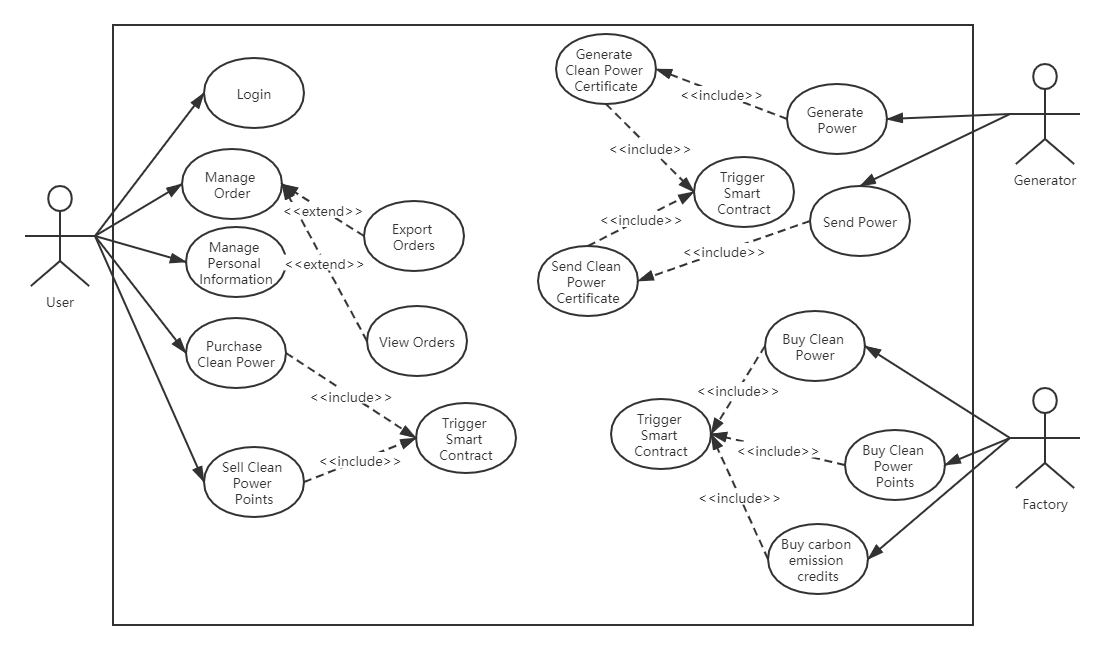
\includegraphics[width=\textwidth]{img/Usecaseforsummerproject.png}
    \caption{Use case diagram of the system}
    \label{fig:usecase}
\end{figure}

\section{Class Diagram}
% 通过类图,系统的实体之间的关系可以被清晰的观察到,本项目定义了用户,发电终端,清洁电力证书,订单,礼物,清洁电力积分,清洁电力等实体,类之间的关系和类的具体结构被\fref{fig:classdiagram}详细的表示了出来。
The relationship between the entities of the system can be clearly observed through the class diagram. This project defines entities such as user, generation terminal, clean power certificate, order, gift, clean power credit, clean power, and so on. The relationship between the classes and the specific structure of the classes are represented in detail by \fref{fig:classdiagram}.
\begin{figure}[!htb]
    \centering
    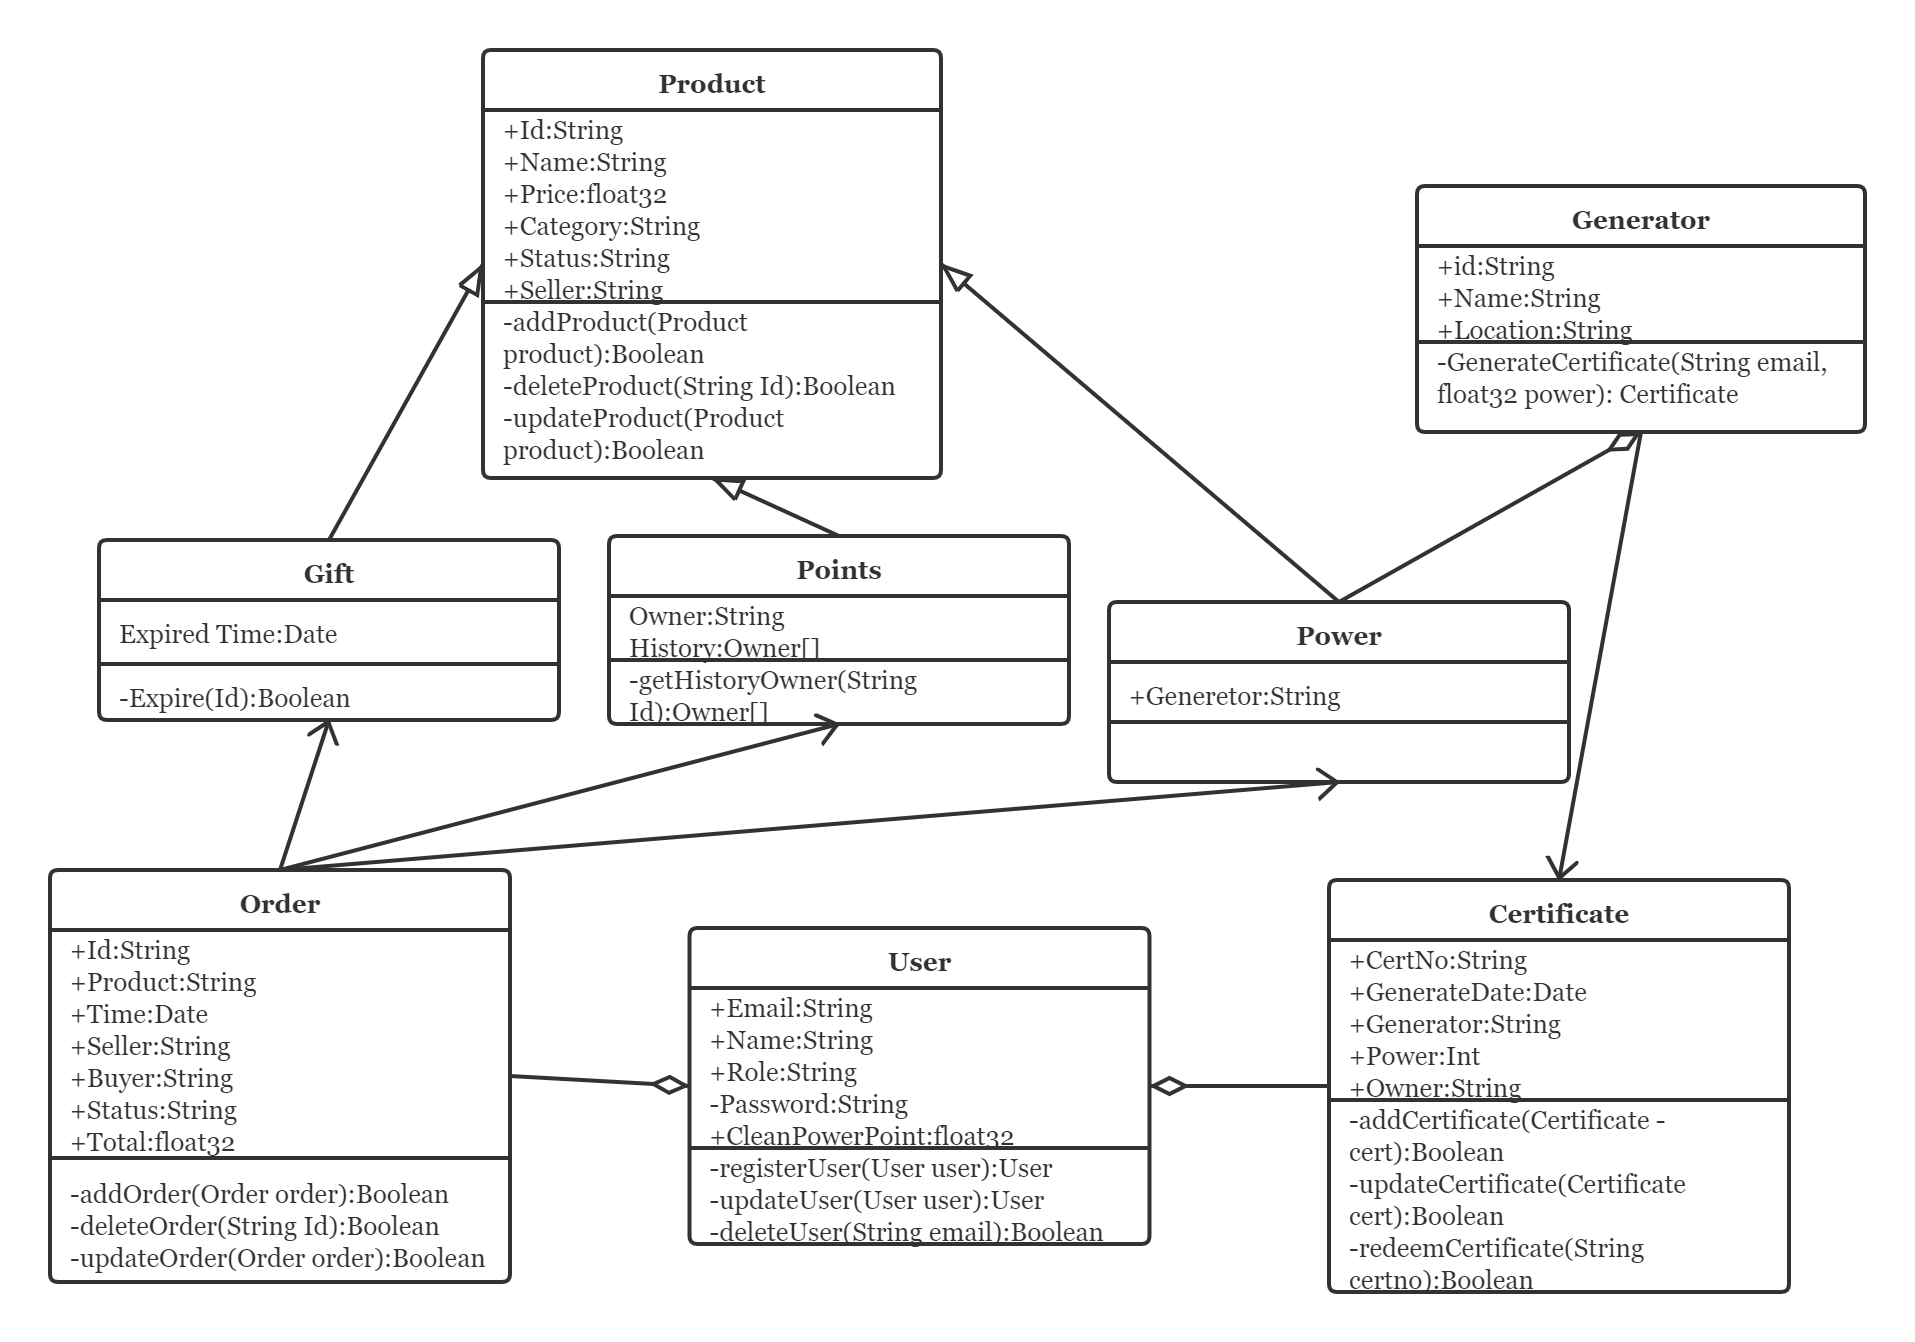
\includegraphics[width=\textwidth]{img/classdiagram.png}
    \caption{Class diagram of the system}
    \label{fig:classdiagram}
\end{figure}

\section{System Architecture}
% 为了能够快速高效的进行系统开发,在确定了系统用例以及实体之间关系之后,需要进行系统的架构设计,以便选择合适的实施方法,实施平台,从而进入实际的开发阶段,本项目选用Browser/Client结构,通过浏览器对区块链进行访问,使用Nodejs,Express,MongoDB,React实现传统的数据操作逻辑,使用Golang进行智能合约开发,将传统数据操作逻辑与智能合约通过Restful Api进行连接,最后对区块链进行操作。详细的系统结构如\fref{fig:sysarchtecture}所示。
In order to be able to develop the system quickly and efficiently, after determining the system use cases and the relationship between entities, the system architecture design is needed in order to select the appropriate implementation method and implementation platform, so as to enter the actual development phase, this project chooses Browser/Client structure, accessing the blockchain through the browser, choosing Nodejs, Express, MongoDB, React (MERN technology stack) to implement the traditional data operation logic, use Golang for smart contract development, connect the traditional data operation logic with the smart contract through Restful Api, and finally the smart contract will operate on the blockchain. The detailed system structure is shown in \fref{fig:sysarchtecture}.
\begin{figure}[!htb]
    \centering
    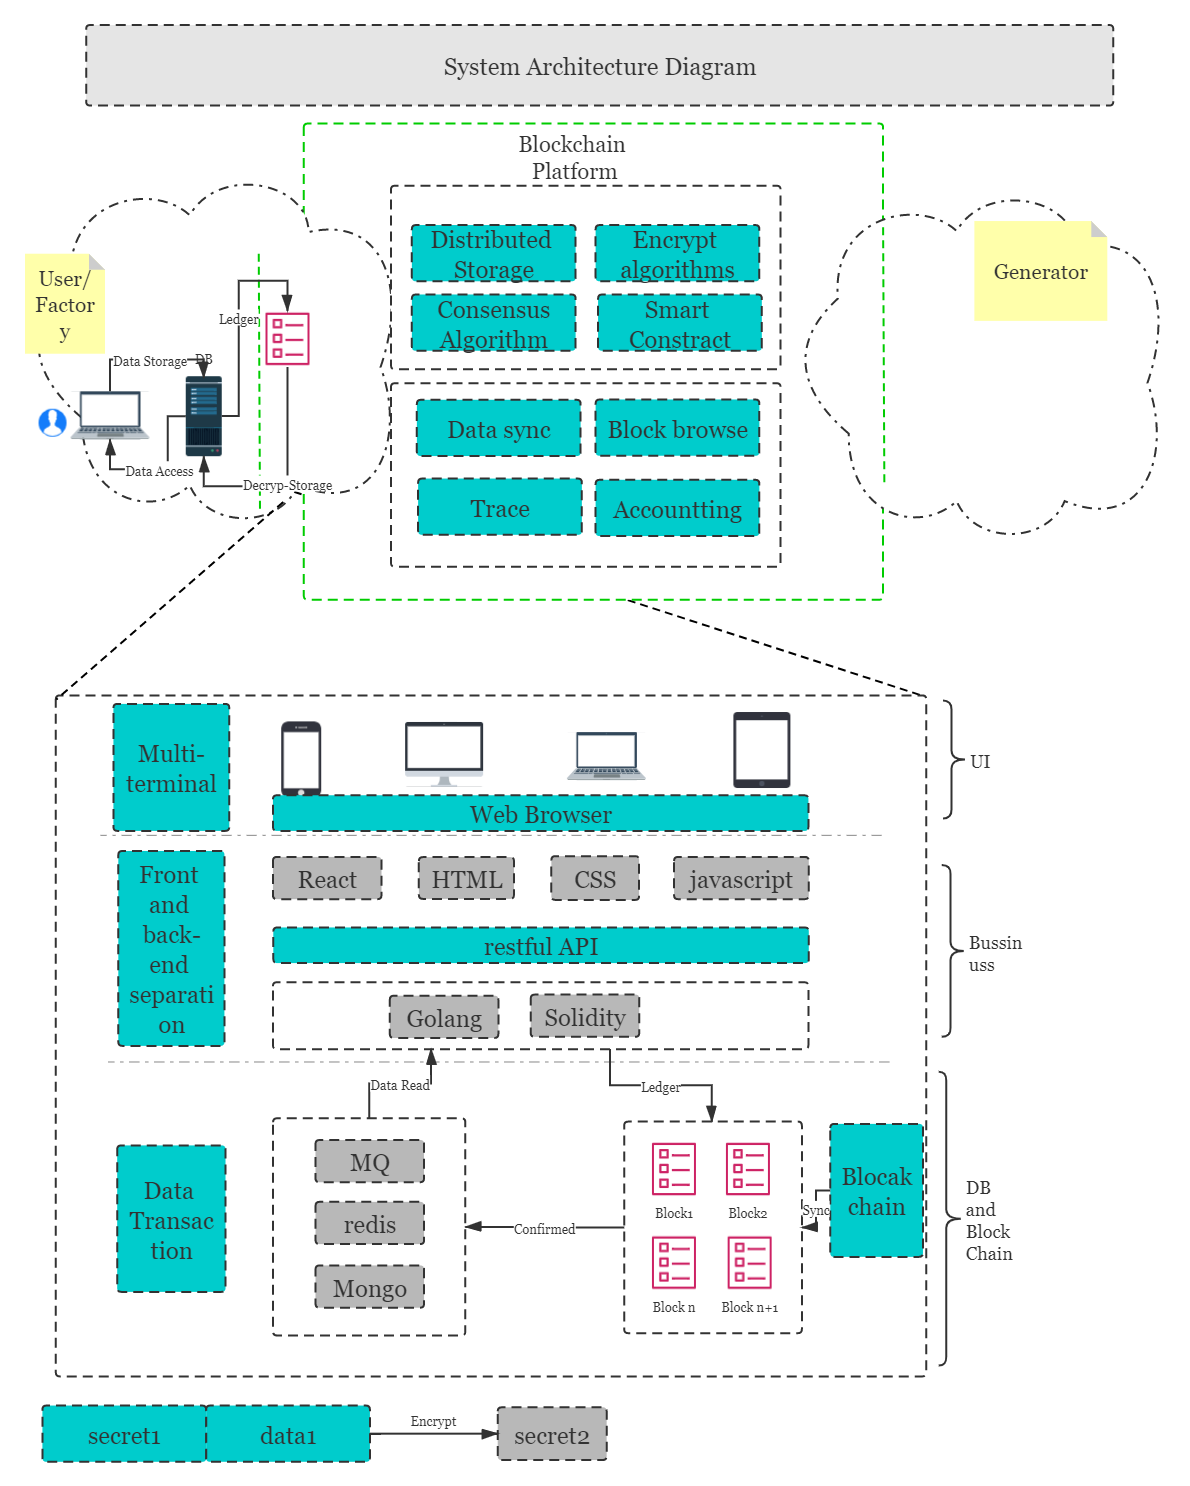
\includegraphics[width=.8\textwidth]{img/Architecture.png}
    \caption{System Architecture of the system}
    \label{fig:sysarchtecture}
\end{figure}



\chapter{Implementation}
% 确定系统功能与架构之后,则需要进行实际的项目开发阶段,在这个阶段会进行开发工具选择,区块链网络设计与搭建,开发平台部署,编码等活动,本节会对这些实施阶段的过程进行简要描述。
In this chapter, activities such as development tool selection, blockchain network design and construction, development platform deployment, and coding are undertaken, and the process of these implementation phases will be briefly described.

\section{Development SDK and Tools Selection}
% 在项目开发中用到的开发工具和SDK都在\tref{Table:toolsused}列出
The development tools and SDKs used in the project development are listed in \tref{Table:toolsused}
\begin{table}[!htb]
\resizebox{\textwidth}{!}{
\begin{tabular}{lll}
\toprule
\textbf{Name}                & \textbf{Usage}                                 & \textbf{Version} \\ \midrule
Virtual Box                  & Run the virtual machine                        & 6.1              \\ \midrule
Vagrant                      & Setup development environment quickly          & 2.2.14           \\ \midrule
Git                          & Project synchronization and collaborative work & 2.30.1           \\ \midrule
Docker                       & Run the blockchain nodes                       & 20.10.8          \\ \midrule
Docker-Compose               & Define Multi-Container                         & 1.29.2           \\ \midrule
Hyper Ledger Fabric          & Build the blockchain network                   & 2.2              \\ \midrule
CouchDB                      & Store the data and state in the blockchain     & 1.4.1            \\ \midrule
Golang                       & Develop the smart contracts                    & 1.16             \\ \midrule
NPM                          & Manage the software and packages               & 6.14.14          \\ \midrule
NodeJS                       & Runtime of the backend application             & 14.17.5          \\ \midrule
Express                      & Server of the backend applicaiton              & 4.17.1           \\ \midrule
MongoDB                      & Storage of insignificant data                  & Online           \\ \midrule
React                        & UI implementation                              & 16.13.1          \\ \midrule
Visual Studio Code           & Use for code                                   & 1.59.1           \\ \midrule
Hyper Ledger Fabric Explorer & Monitor the blockchain                         & 1.1.8           \\
\bottomrule
\end{tabular}
}
\caption{Tools used in project}
\label{Table:toolsused}
\end{table}

\section{Blockchain Network Design}
% 本项目所建立的区块链网络由两个组织组成,每个组织分别拥有两个节点,这两个组织公用一个通道和四个排序节点。网络的结构如\fref{fig:networkarc}所示。
The blockchain network created in this project consists of two organizations, each with two nodes respectively, and these two organizations share a common channel and four raft consensus sorting nodes. The structure of the network is shown in \fref{fig:networkarc}.

\begin{figure}[!htb]
    \centering
    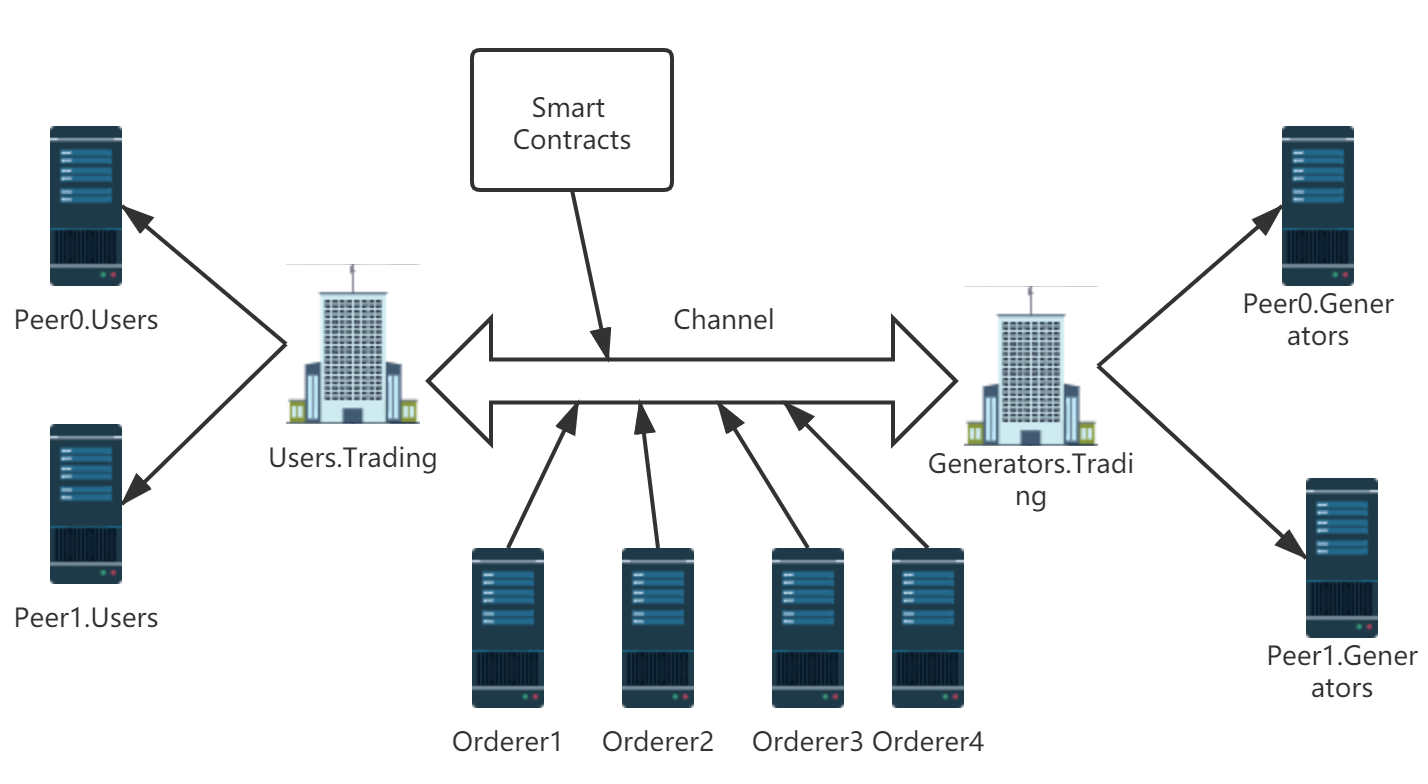
\includegraphics[width=.7 \textwidth]{img/networkarc.png}
    \caption{Blockchain network architecture of the system}
    \label{fig:networkarc}
\end{figure}

% 在设计好网络之后,需要依照Hyper Ledger Fabric的官方文档编写命令脚本对各个组织以及网络节点进行证书,密钥以及创世区块的生成活动,命令运行成功后可以生成项目所建立的区块链网络的基础设施文件,具体的文件结构如\fref{fig:networkfilestructure}.
After designing the network, it is necessary to write command scripts to generate certificates, keys and genesis blocks for each organization and network node according to the official documentation of Hyper Ledger Fabric, and the command will generate the infrastructure files of the blockchain network established by the project after running successfully, as shown in \fref{fig:networkfilestructure}.
\begin{figure}[!htb]
    \centering
    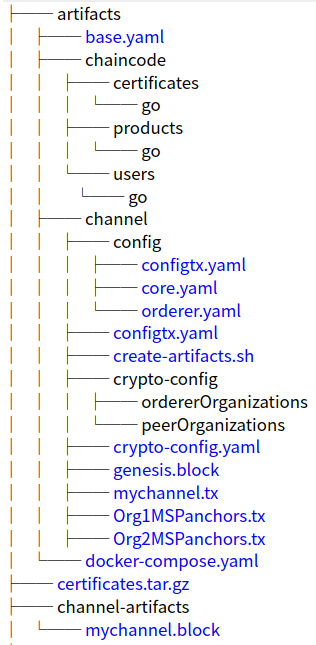
\includegraphics[width = .3 \textwidth]{img/artifacts.png}
    \caption{File structure of the blockchain network}
    \label{fig:networkfilestructure}
\end{figure}

\section{Smart Contracts Design}
% 在Hyper Ledger Fabric中,智能合约被称为链码,本项目的链码使用Golang编写,主要包含处理用户数据和清洁电力证书的智能合约,用户智能合约流程图显示在\fref{fig:flowUser}中,清洁电力证书智能合约流程图由\fref{fig:flowCert}表示。


In Hyper Ledger Fabric, smart contracts are called chain code. The chain code of this project is written in Golang and contains mainly smart contracts for handling user data and clean power certificates. Program flow of the user and clean power certificates contract is shown in \fref{fig:flowUser} and \fref{fig:flowCert}.
\begin{figure}[H]
    \centering
    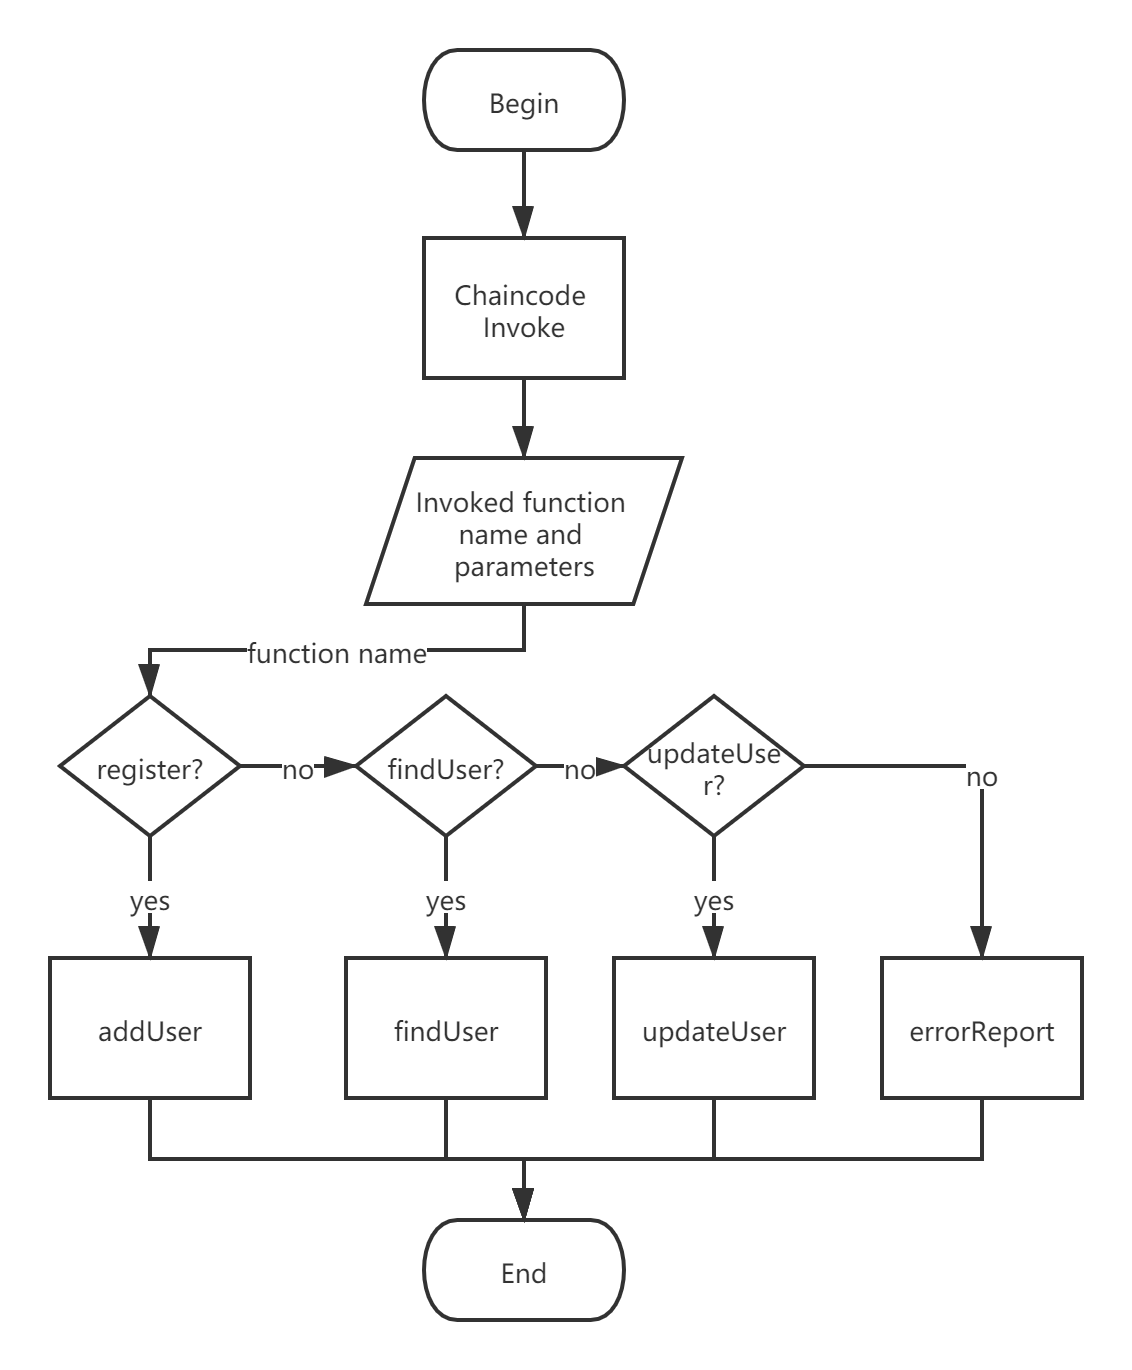
\includegraphics[width=.5 \textwidth]{img/flowUser.png}
    \caption{Program flow of chaincode for users}
    \label{fig:flowUser}
\end{figure}

\begin{figure}[H]
    \centering
    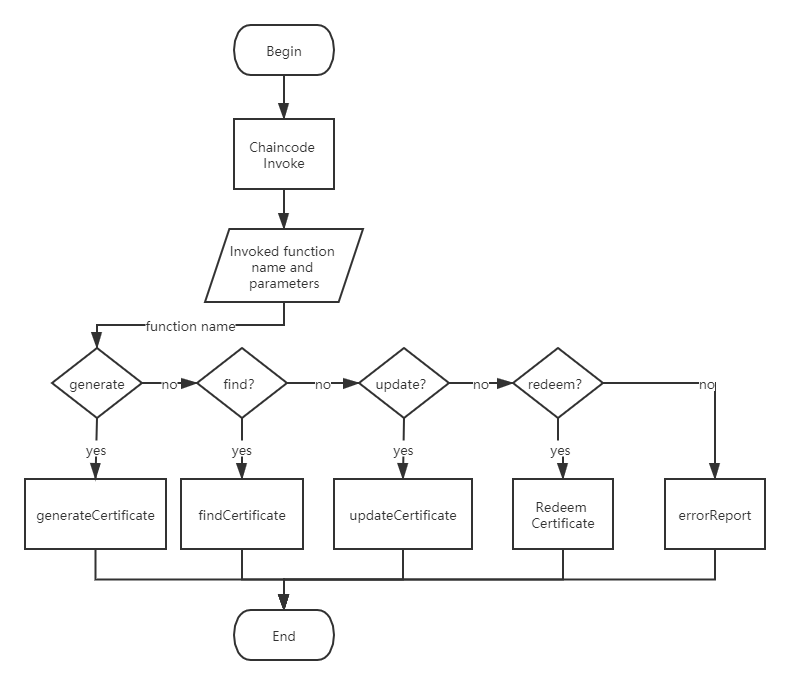
\includegraphics[width=.6 \textwidth]{img/flowCert.png}
    \caption{Program flow of chaincode for clean power certificate}
    \label{fig:flowCert}
\end{figure}

\section{Start Blockchian Network and Deploy Smart Contracts}
% 完成了区块链网络的配置以及智能合约的编写后,就需要开启区块链网络并将智能合约部署到网络中的通道上,通过编写Shell脚本,完成批处理操作后,区块链网络在Docker容器中成功的运行,\fref{fig:dockerps}表示了证书认证节点,排序节点,CouchDB节点以及组织中的四个节点都正常的启动了。
After completing the configuration of the blockchain network and writing the smart contracts, it is time to launch the blockchain network and deploy the smart contracts to the channel in the network. By writing shell scripts and completing batch operations, the blockchain network runs successfully in the Docker container,\fref{fig:dockerps} indicates that the certificate authentication node, the sorting node, the CouchDB node and the four nodes in the organization are started properly.\fref{fig:installchaincode} shows the chaincode has been installed correctly.
\begin{figure}[!htb]
    \centering
    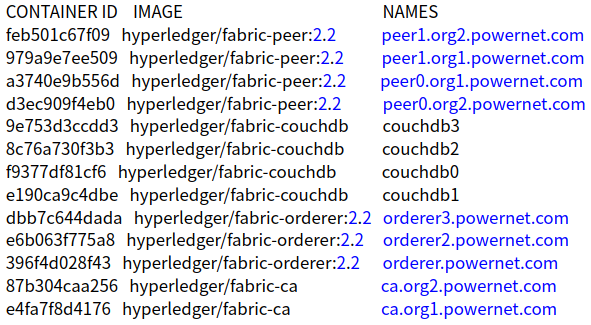
\includegraphics[width=\textwidth]{img/dockerps.png}
    \caption{Docker container process list after starting network}
    \label{fig:dockerps}
\end{figure}

\begin{figure}[!htb]
    \centering
    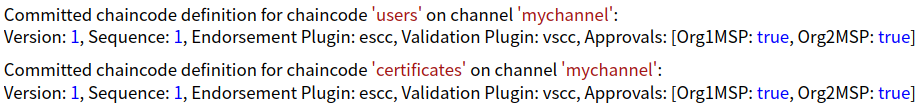
\includegraphics[width=\textwidth]{img/installChaincode.png}
    \caption{Result of installing chaincode}
    \label{fig:installchaincode}
\end{figure}

\section{Coding and realization}
% 智能合约被安装在区块链网络中后,可以将进行UI和后台的开发,实现业务逻辑,本项目使用NodeJS,和React作为实现工具,实现了\fref{fig:login}中的用户登录功能,用户输入邮箱和密码即可登入系统进行操作,也实现了\fref{fig:powermarket},\fref{fig:giftmarket},\fref{fig:pointmarket}中的清洁电力,清洁电力礼品,清洁电力积分交易市场,用户可以在这三个市场进行相应的物品交易,同时还实现了\fref{fig:certmanage}中的清洁能源证书管理功能,可以将清洁能源证书兑换为清洁能点积分。另外的,系统中还实现了用户注册,用户信息管理,订单管理等功能模块没有展现在本文中。
After the smart contract is installed in the blockchain network, the UI and backend development can be carried out to implement the business logic. This project uses NodeJS and React as implementation tools to implement the user login function in \fref{fig:login}, where users can login to the system by entering their email and password, and also implement the clean power, clean power gifts, and clean power points trading markets in \fref{fig:powermarket},\fref{fig:giftmarket}, and \fref{ fig:pointmarket} in the clean power, clean power gifts, clean power points trading market, users can trade the corresponding items in these three markets, and also realized \fref{fig:certmanage} in the clean power certificate management function, can be redeemed clean power certificates for clean power points. In addition, the system also implements user registration, user information management, order management and other functional modules that are not displayed in this paper.
\begin{figure}[!htb]
    \centering
    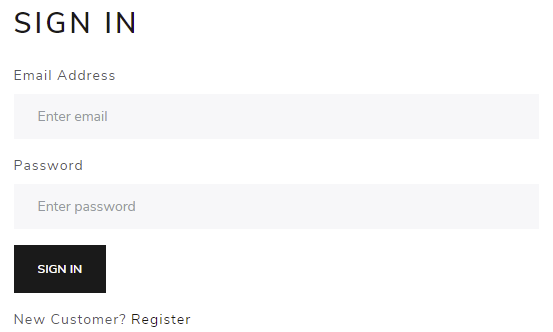
\includegraphics[width=.6 \textwidth]{img/login.png}
    \caption{Login page of the project}
    \label{fig:login}
\end{figure}
\begin{figure}[!htb]
    \centering
    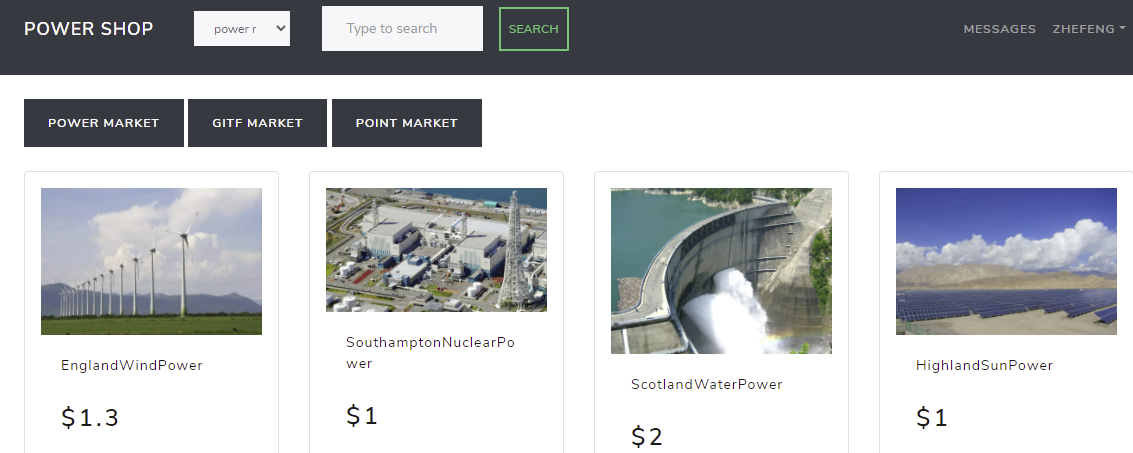
\includegraphics[width= .7\textwidth]{img/powermarket.png}
    \caption{Clean power market of the project}
    \label{fig:powermarket}
\end{figure}
\begin{figure}[!htb]
    \centering
    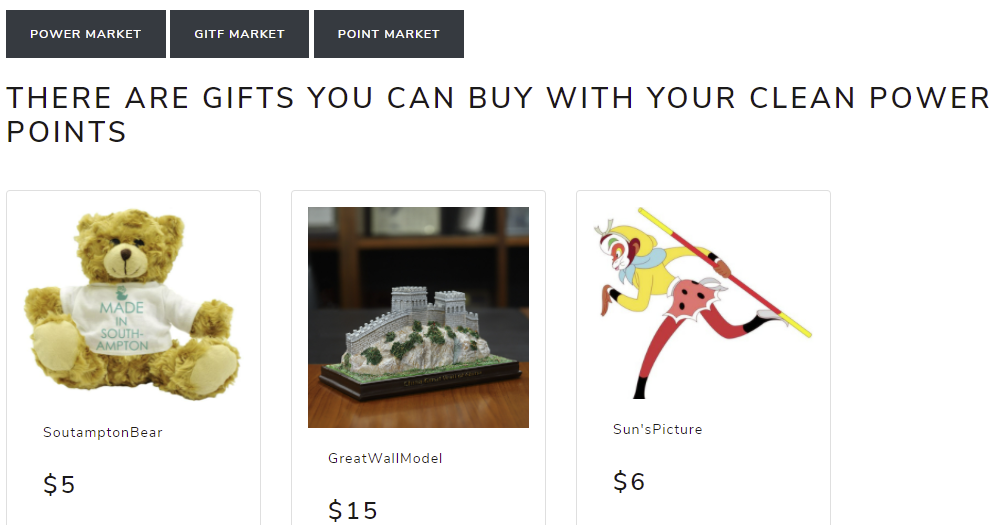
\includegraphics[width=.7 \textwidth]{img/giftmarket.png}
    \caption{Clean power market of the project}
    \label{fig:giftmarket}
\end{figure}
\begin{figure}[!htb]
    \centering
    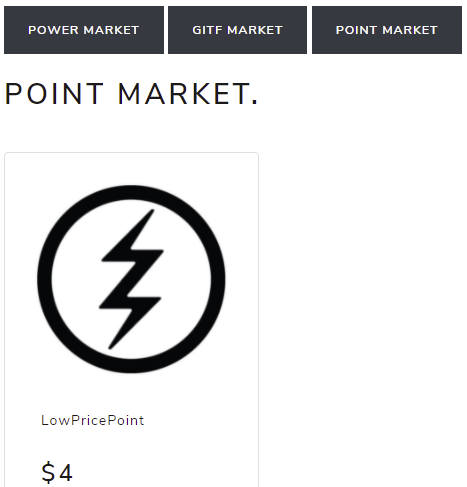
\includegraphics[width= .7 \textwidth]{img/pointmarket.png}
    \caption{Clean power point market of the project}
    \label{fig:pointmarket}
\end{figure}
\begin{figure}[!htb]
    \centering
    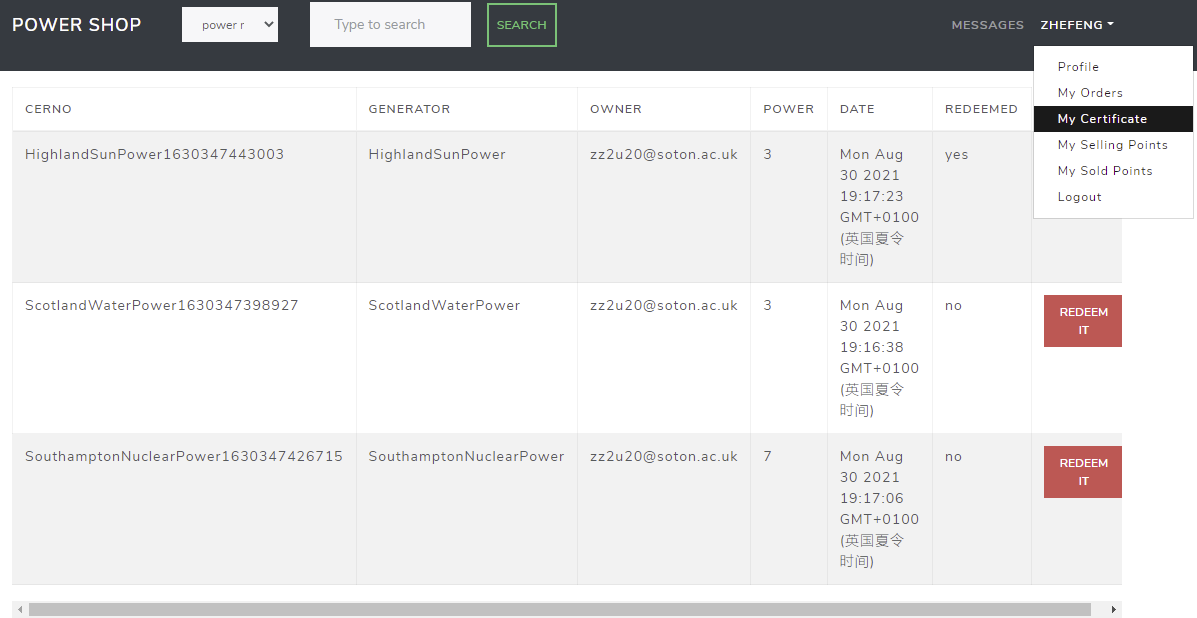
\includegraphics[width=\textwidth]{img/certificateManage.png}
    \caption{Certificates management of the project}
    \label{fig:certmanage}
\end{figure}


\chapter{Software Testing and Validation} \label{chapter:testing}
% 在软件开发完成之后需要对软件进行测试以发现软件存在的错误和缺陷,进而对软件进行修补和完善,在测试完成之后需要对软件进行验证以检查软件表现是否符合需求文档的预期。
% 本文使用Mocha和Chai对项目的用户,市场,以及交易场景Api进行自动测试,通过模拟前端对后台的请求获得后台返回的数据,将返回的数据与预期的数据进行对比,如果数据一致则说明Api工作正确。自动测试结果如\fref{fig:testapi}所示,结果显示本项目的Api工作正常。
After the software is completed, the software needs to be tested to find bugs and defects, and then the software needs to be fixed and improved, followed by validation to check whether the software performs as expected in the requirements document. This chapter will display the result of testing and validation.

In this paper, Mocha and Chai are used to automatically test the Apis for user, market, and transaction scenarios of the project. The result of the automatic test is shown in \fref{fig:testapi}.
\begin{figure}[!htb]
    \centering
    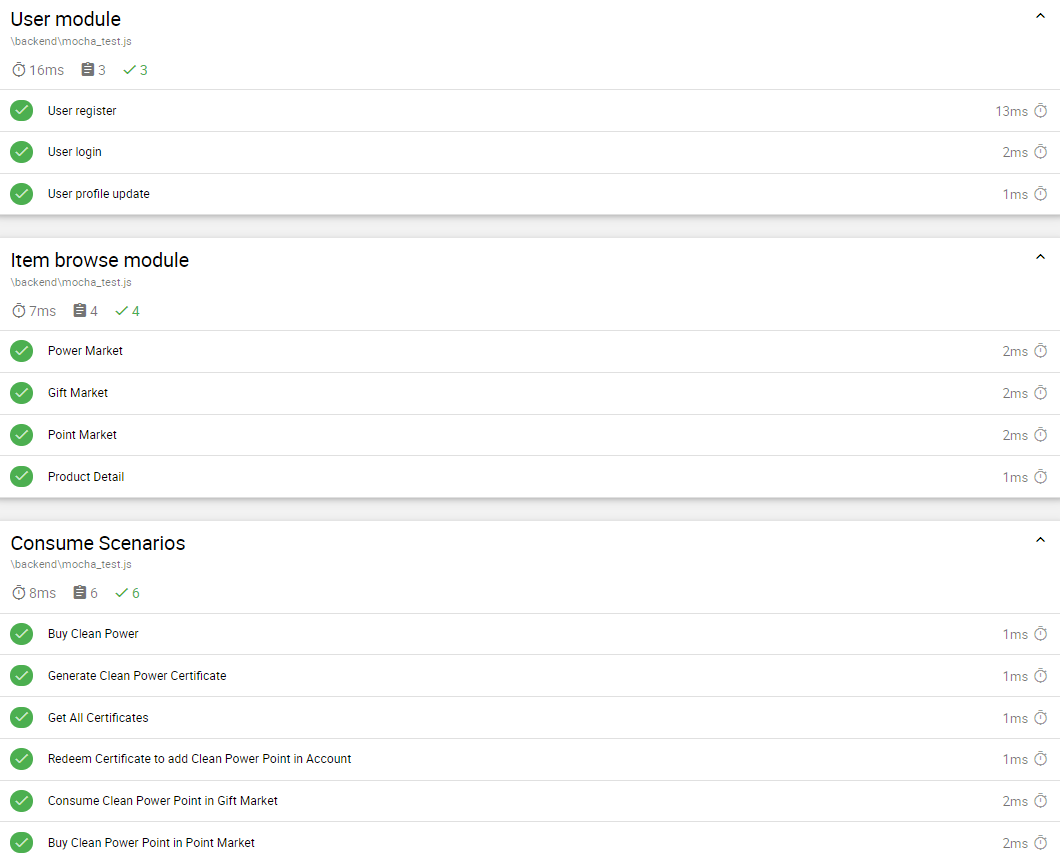
\includegraphics[width=.8 \textwidth]{img/testresult.png}
    \caption{Testing result of Apis}
    \label{fig:testapi}
\end{figure}

% 本文通过Hyper Ledger Explorere进行软件验证,在每一项操作完成之后对区块链数据进行查看,\fref{fig:dataoverview}和\fref{fig:transaction}分别代表了区块链数据总览以及交易信息查看,验证结果显示本项目符合需求文档要求。
Hyper Ledger Explorere is used to validate the software in this project, and the blockchain data is viewed after each operation is completed, \fref{fig:dataoverview} and \fref{fig:transaction} represent the blockchain data overview and transaction information view respectively. The validation results show that this project meets the requirements of the requirement document.
\begin{figure}[!htb]
    \centering
    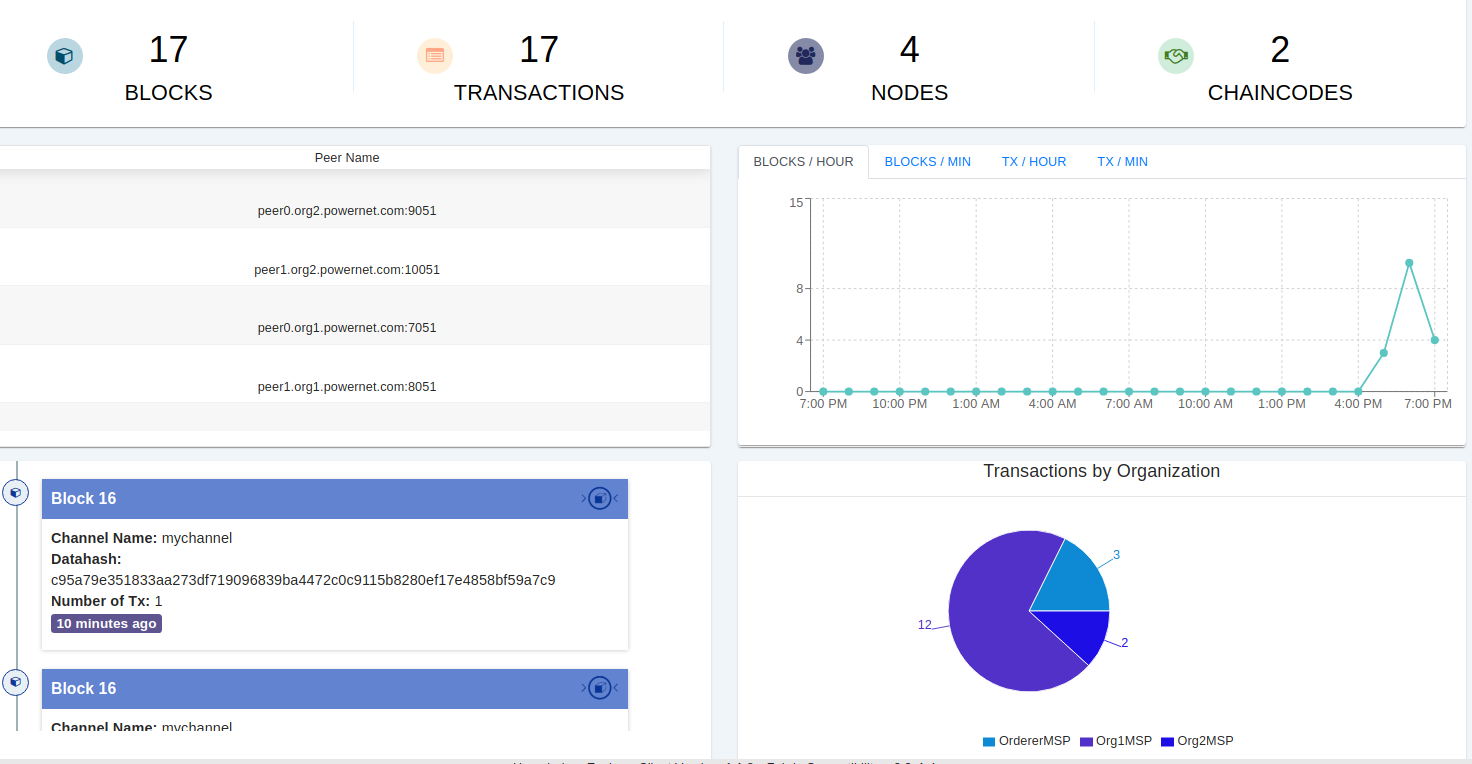
\includegraphics[width= \textwidth]{img/overview.png}
    \caption{System data overview}
    \label{fig:dataoverview}
\end{figure}
\begin{figure}[!htb]
    \centering
    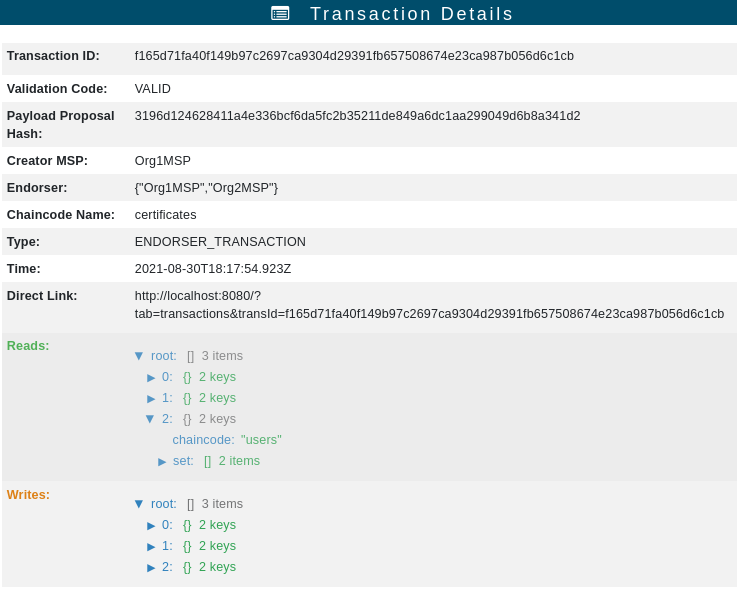
\includegraphics[width=.9 \textwidth]{img/transaction.png}
    \caption{Transaction monitoring}
    \label{fig:transaction}
\end{figure}

\chapter{Evaluation}
This chapter is an evaluation of the project management and result of this project.
\section{Project Management and Schedule}
% 本项目通过学校Git进行项目管理,将项目甘特图转化为了Git中的Milestone,如图\fref{fig:milestone}所示,并且将项目分解为不同的需求和步骤列在了项目的Board中,如图fref{fig:board}所示。项目进度严格按照Miles中的时间线进行,如期完成了文档,设计,开发以及测试活动。
The project was managed through the university-owned Git. The project Gantt chart shown in \fref{fig:gannt} was converted into a Milestone in Git, as shown in figure \fref{fig:milestone}, and the project was broken down into different requirements and steps listed in the project board, as shown in figure \fref{fig:board}. The project progressed strictly according to the timeline in Milestone, and completed the documentation, design, development, and testing activities on schedule.
\begin{figure}[H]
    \centering
    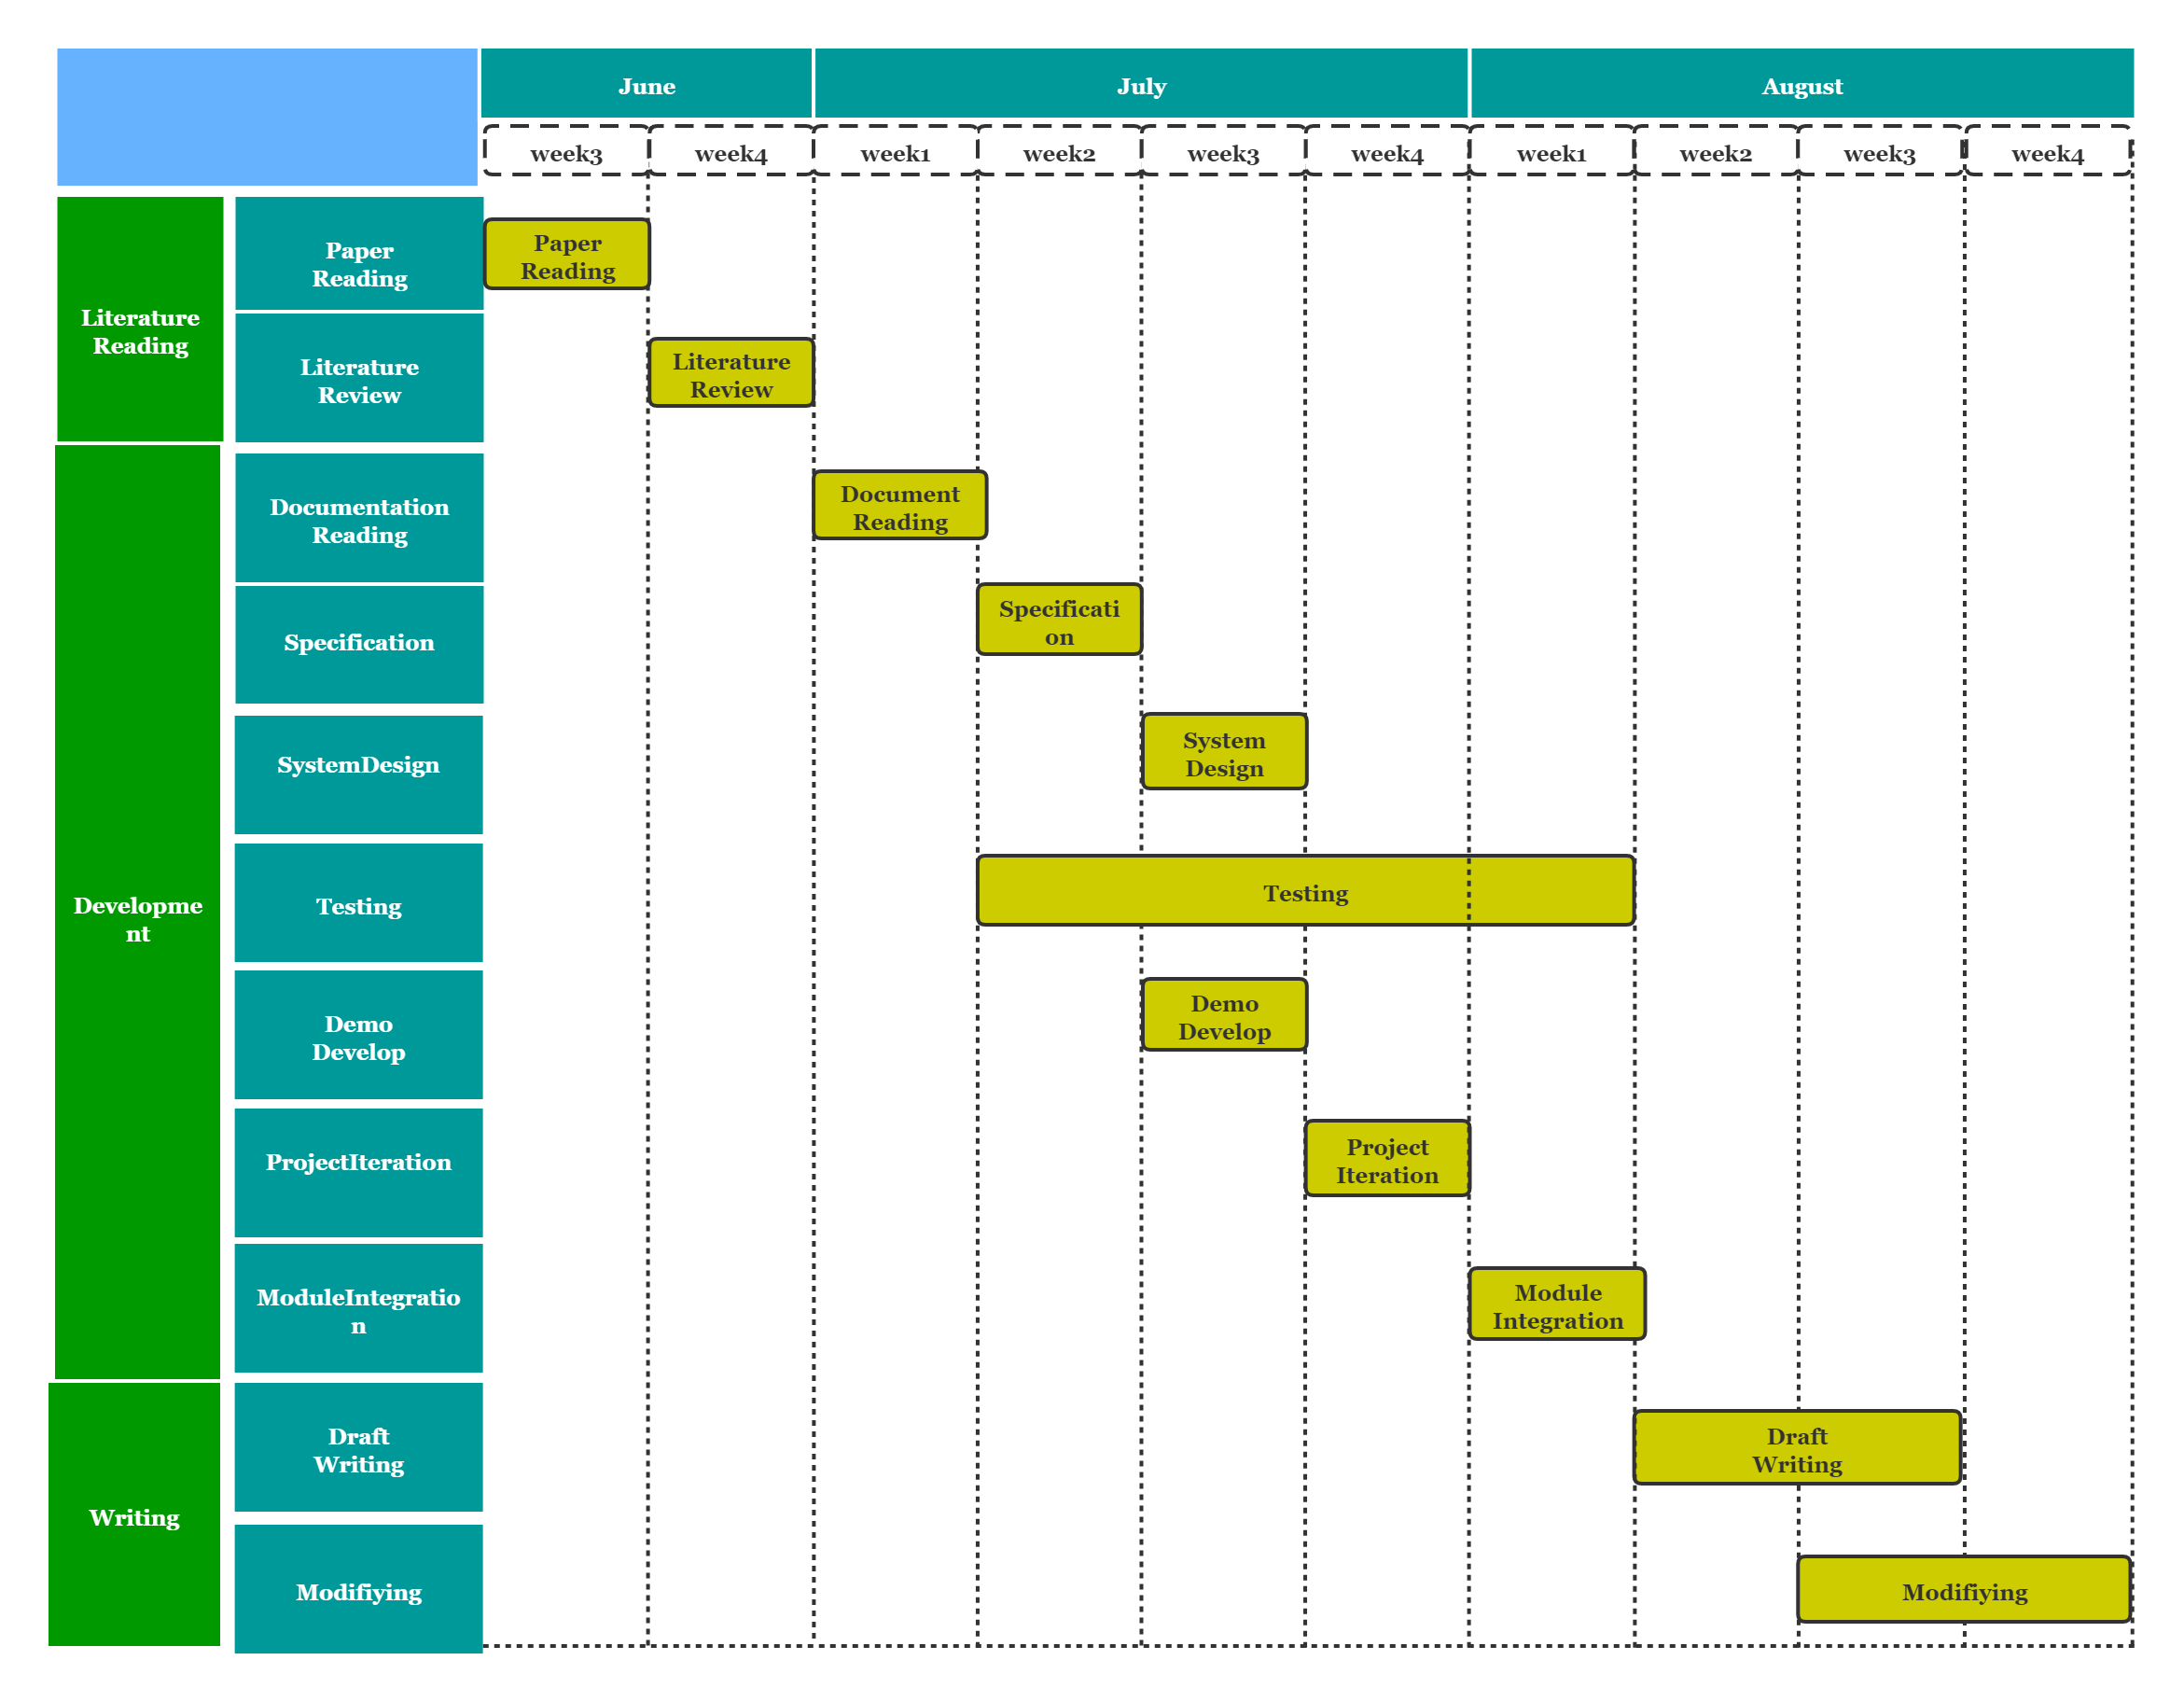
\includegraphics[width= .7 \textwidth]{img/gant.png}
    \caption{Gannt chart of the project}
    \label{fig:gannt}
\end{figure}
\begin{figure}[H]
    \centering
    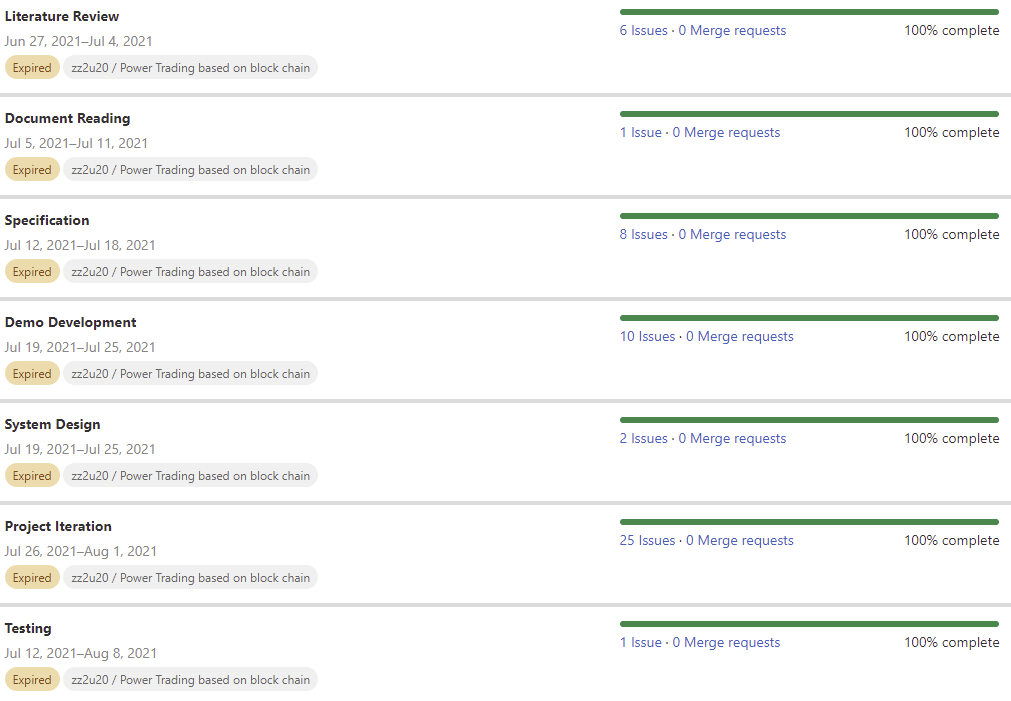
\includegraphics[width= .8 \textwidth]{img/milestone.png}
    \caption{Milestone of the project}
    \label{fig:milestone}
\end{figure}
\begin{figure}[H]
    \centering
    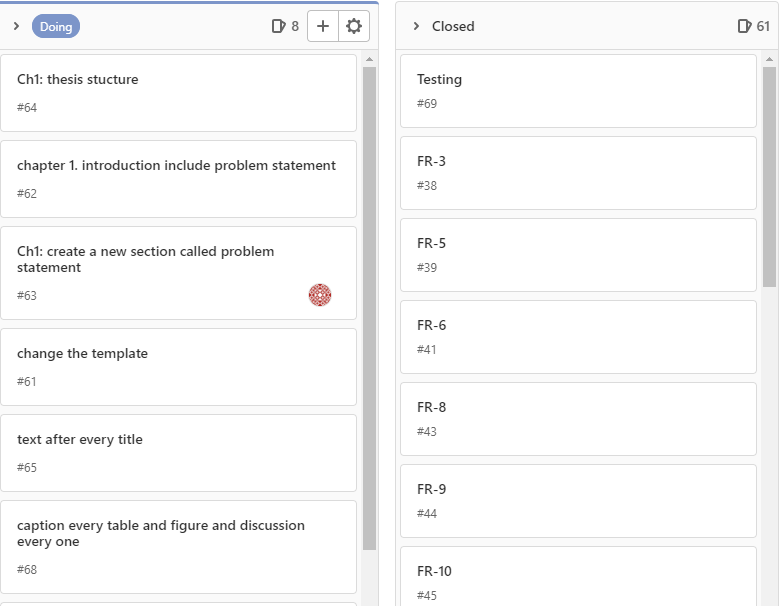
\includegraphics[width= .6 \textwidth]{img/board.png}
    \caption{Task board of the project}
    \label{fig:board}
\end{figure}

\section{Features of Project}
% 正如文献综述所说,目前市场并没有适合个人投资者进入的且能够联通清洁电力交易市场和碳排放市场的平台或者应用,因此本项目弥补了一个市场空白,根据软件实施,测试和验证章节的结果,本项目实现了一个有着界面简单,用户体验友好,交易确认速度快,稳定可靠的清洁能源交易平台。
As stated in the literature review, there is no platform or application for individual investors to enter the market that can link the clean power trading market and the carbon market, so this project fills a gap in the market. Based on the results of the software implementation, testing and validation chapter, this project achieves a clean power trading platform with features of simple interface, user-friendly experience, fast transaction confirmation, and stable and reliable.
%% ----------------------------------------------------------------
%% Conclusions.tex
%% ---------------------------------------------------------------- 
\chapter{Conclusions and Reflection} \label{Chapter: Conclusions}
% 对于普通用户而言,本系统实现了用户自主注册,自主进行清洁能源电力购买并自主将清洁能源电力证书兑换为清洁能源积分的功能,同时用户可以用清洁能源电力积分兑换礼品市场中的礼品,另外,用户的清洁能源电力积分也可以用来相互交易。用户的功能需求和安全需求以及性能需求都符合需求文档的描述。对于管理员而言,可以随时监视系统的订单,用户信息,符合用户故事中对管理员的描述。对于发电终端而言,本系统设计了可以自动颁发证书的智能合约,因此也完成了需求文档的要求。值得提出的是系统在误操作和实用性方面仍有较大可提升空间,距离实际的投入消费领域还有很大差距,需要细化需求,精细开发。
% 需要指出的是,因为气候变化以及能源问题严峻,本项目所提出的碳排放市场普及化以及碳排放市场与其他领域挂钩是一个很有可能被实现的设想,因此本项目很可能未来拥有很高的社会以及商业价值
For general users, the system implements the function that users can independently register, independently make clean power purchases and independently redeem clean power certificates for clean power points, while users can exchange clean power points for gifts in the gift market, in addition, the clean power points of users can also be used to trade with each other. The functional and security requirements and performance requirements of the users are in accordance with the requirements document. For administrators, the system can be monitored at any time for orders, user information, in line with the description of administrators in the user story. For the power generator terminal, the system is designed with a smart contract that can automatically issue certificates, so it also fulfills the requirements of the requirement document. It is worth to propose that the system still has a large space for improvement in terms of misuse and practicality, and there is still a big gap from the actual input to the consumer field, which needs to refine the requirements and fine development.

It is important to note that the idea of universalizing the carbon market and linking it to other fields, as proposed in this project, is a very likely one to be realized because of the seriousness of climate change and energy issues, and therefore this project is likely to have a high social and commercial value in the future.
\section{Future Work}
% 与区块链相同,人工智能近些年也与许多传统领域开始开始了逐步的结合,并且效果不凡,因此未来可以将人工智能技术与本项目进行结合,开发出一个基于区块链的智能清洁电力和碳排放交易系统,使用算法博弈论方法为系统设计智能代理,为交易系统构建一个市场价格机制,使得交易系统的所有利益相关者获得最优收益,同时利用机器学习或强化学习算法分析用户数据,对用户进行画像从而提高用户体验;对于区块链网络底层,可以使用负载均衡技术,在分布式网络运行成本和用户交易速度之间取得最优平衡;对于前后端开发,可以使用Golang或者Java Spring框架替换NodeJS来实现高并发系统;对于拓展性而言,未来可以将系统开发成标的物可插拔的形式,即可以在需要的时候将诸如公共交通票据,自行车行程等项目方便快速的接入碳排放市场。总之,在这个领域,有很多方向都有很大的可能性。
Similar to blockchain, artificial intelligence has also started to gradually combine with many traditional fields in recent years, and the effect is extraordinary. Therefore, artificial intelligence technology can be combined with this project in the future to develop an intelligent clean power and carbon emission trading system based on blockchain, using algorithmic game theory methods to design intelligent agents for the system and build a market price mechanism for the trading system, so that an optimal revenue can be obtained by all stakeholders of the trading system. At the same time, machine learning or reinforcement learning algorithms can be used to analyze user data and profile users to improve user experience; for the underlying blockchain network, load balancing technology can be used to achieve an optimal balance between distributed network operation cost and user transaction speed; for front and back-end development, Golang or Java Spring framework instead of NodeJS to achieve a highly concurrent system; for expandability, the system can be developed into a pluggable form of the target object in the future, which means that items such as public transportation tickets and bicycle trips can be easily and quickly connected to the carbon emission market when needed. In short, there are many directions with great possibilities in this field.
\appendix
\backmatter
\bibliographystyle{unsrt}
\bibliography{ECS}
\end{document}
%% ----------------------------------------------------------------
